

\section{Introduction}


Bayesian computation lies at the heart of many machine learning models in both academia and industry \cite{bishop2006pattern}. Thus, it is of major importance to develop efficient approximation techniques that tackle the intractable integrals that arise in large scale Bayesian inference and prediction problems \cite{gelman2013bayesian}. 

Recent developments in Bayesian techniques applied to large scale datasets and deep models include variational based approaches such as \emph{Automatic Differentiation Variational Inference} (ADVI) \cite{blei2017variational}, and \emph{Stein Variational Gradient Descent} (SVGD)  \cite{liu2016stein} or sampling approaches such as \emph{Stochastic Gradient Markov Chain Monte Carlo} (SG-MCMC) \cite{ma2015complete}. While variational techniques enjoy faster computations, they rely on optimizing a family of posterior approximates that may not contain the actual posterior distribution, potentially leading to severe bias and underestimation of uncertainty, \cite{pmlr-v80-yao18a} or \cite{48127}. SG-MCMC methods have been used in a wide range of real-world tasks, such as in computer vision settings \cite{7780980} or in recommendation systems via matrix factorization \cite{7952555}.%In addition, though current work focuses on creating richer families of variational posteriors, it is not clear how to choose this variational family. 

There has been recent interest in bridging the gap between variational Bayes and MCMC techniques, see e.g. \cite{zhang2018}, to develop new scalable approaches for Bayesian inference, e.g., \cite{carbonetto2012}.
In this work, we draw on a similitude between the SG-MCMC and SVGD approaches to propose a novel family of very efficient sampling algorithms. 
Any competing MCMC approach should verify the following list of properties as our proposal will do:
\begin{itemize}
    \item \emph{scalability}. For this, we resort to SG-MCMC methods since at each iteration they may be approximated to just require a minibatch of the dataset,
    \item \emph{convergence to the actual posterior}, and
    \item \emph{flexibility}. Since we provide a parametric formulation of the transition kernel, it is possible to adapt other methods such as \emph{Hamiltonian Monte Carlo}, \cite{neal2011mcmc}, or the Nos\'e-Hoover thermostat method, \cite{ding2014bayesian}.
\end{itemize}
% MUY LARGO PA WORKSHOP: 
% Any competing MCMC algorithm should verify the following list of desiderata:
% \begin{enumerate}
% \item Scalability. A standard MCMC iteration requires a full dataset sweep to compute the acceptation probability, which renders its application to large scale datasets intractable. Thus, we resort to SG-MCMC methods since at each iteration they may be approximated to just require a minibatch of the dataset.
% \item Convergence to the true posterior. The dynamics of the underlying stochastic differential equation should converge to the exact posterior. SG-MCMC introduces a discretization of the previous SDE that induces some bias. However we shall see that it is controllable and smaller than in variational methods. 
% \item Flexibility. Since, we provide a parametric formulation of the transition kernel, we can adapt other methods such as \emph{Hamiltonian Monte Carlo} \cite{chen2014stochastic} or the Nosé-Hoover thermostat method. \cite{ding2014bayesian}
% \end{enumerate}

Our contributions are summarized as follows. First, we provide a unifying hybrid scheme of SG-MCMC and SVGD algorithms satisfying the previous list of requirements. Second, and based on the previous connection, 
we develop new SG-MCMC schema that include repulsive forces between particles and momentum acceleration. Finally, we show how momentum-based extensions of SGD can be incorporated into our framework, leading to new samplers which benefit from both momentum acceleration and repulsion between particles for better exploration of complex posterior landscapes, therefore providing a very competitive scheme. 

Figure \ref{fig:diagram} provides a diagram of our proposal. Starting with SGD, one can add a carefully crafted noise term to arrive at the simplest SG-MCMC sampler, SGLD. Then, one can add repulsion between particles to speed-up the mixing time, leading to SGLD+R, our first contribution (Section \ref{sec:framework}). On top of that, we can further augment the latent space with momentum variables, leading to the Adam+NR sampler, our second proposed sampler (\ref{sec:momentum}).

After an overview of posterior approximation methods in Section \ref{sec:back}, we propose our framework in Section \ref{sec:framework}.
Section \ref{sec:experiments} discusses relevant experiments showcasing the benefits of our proposal. Finally, Section \ref{sec:conclusion} sums up our contributions and highlight several open problems.


\begin{figure}[!h]
    \centering
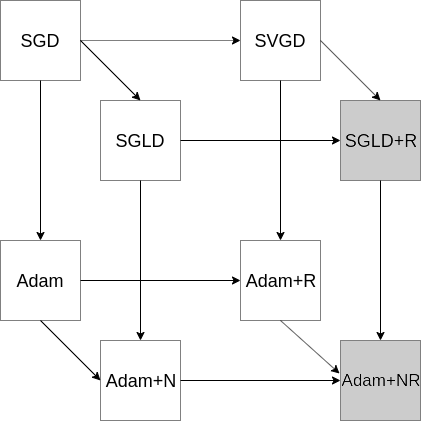
\includegraphics[width=0.4\textwidth]{img/sgmcmc}
    \caption{Relationships between samplers. In light gray, our proposed samplers.}\label{fig:diagram}
\end{figure}



\section{Background and related work}\label{sec:back}

Consider a probabilistic model $p(\bm{x}| \bm{z})$ and a prior distribution $p(\bm{z})$ where $\bm{x}$ denotes an observation and $\bm{z} = ( z_1, \ldots, z_d) $ an unobserved $d-$dimensional latent variable or parameter, depending on the context. We are interested in performing inference regarding the unobserved variable $\bm{z}$, by approximating its posterior distribution:
$$
p(\bm{z} | \bm{x}) = \frac{ p(\bm{z})p(\bm{x}| \bm{z}) }{ \int p(\bm{z})p(\bm{x}| \bm{z}) d\bm{z} } = \frac{ p(\bm{z})p(\bm{x}| \bm{z}) }{ p(\bm{x}) } = \frac{p(\bm{z},\bm{x})}{p(\bm{x})}.
$$
Except for reduced classes of distributions like \textit{conjugate priors}, \cite{raiffa1961applied}, the integral $p(\bm{x}) = \int p(\bm{z})p(\bm{x}| \bm{z}) d\bm{z}$ is analytically intractable; no general explicit expressions of the posterior are available. Thus, several techniques have been proposed to perform approximate posterior inference.


\subsection{Inference as sampling}\label{sec:infassamp}

Hamiltonian Monte Carlo (HMC, \cite{neal2011mcmc}) is an effective sampling method for models whose probability is point-wise computable and differentiable. %HMC uses Hamiltonian dynamics to produce minimally correlated proposals by augmenting the state space of the target distribution $p(z| x)$ with a $d-$dimensional vector $\bm{r}$. The resulting joint distribution is:
%$$
%p(z, \bm{r}| x) = p(z| x)p(\bm{r}),\qquad \bm{r} \sim \mathcal{N}(\bm{0}, \bm{I}).
%$$
%HMC employs two proposals, the first one randomizing $\bm{r}$ (to explore the state space) whereas the second one updates both $z$ and $\bm{r}$ 
%simulating the Hamiltonian dynamics defined through 
%$$
%H(z, \bm{r}) = -\log p(z| x) + \bm{r}^\intercal \bm{r}/2.
%$$
HMC requires the exact simulation of a certain dynamical system which can be cumbersome in high-dimensional or large data settings. When this is an issue, \cite{welling2011bayesian} proposed a formulation of a continuous-time Markov process that converges to a target distribution $p(\bm{z} | \bm{x})$. It is based on the Euler-Maruyama discretization of Langevin dynamics:
\begin{eqnarray}\label{eq:sgld}
\bm{z}_{t+1} \leftarrow \bm{z}_{t} - \epsilon_t \nabla \log p(\bm{z}_t,\bm{x})  + \mathcal{N}(\bm{0}, 2\epsilon_t I),
\end{eqnarray}
where $\epsilon_t$ is the step size. The previous iteration uses the gradient evaluated at one data point $\bm{x}$, but we can use the full dataset or mini-batches. Several extensions of the original Langevin sampler have been proposed to increase mixing speed, see for instance \cite{li2016preconditioned,li2016high,li2019communication}.

\cite{ma2015complete} proposed a general formulation of a continuous-time Markov process that converges to a target distribution $\pi(\bm{z}) \propto \exp (-H(\bm{z}))$. It is based on the Euler-Maruyama discretization of the generalized Langevin dynamics:
\begin{align}\label{eq:sgmcmc}
\begin{split}
&\bm{z}_{t+1} \leftarrow \bm{z}_{t} \\ & -\epsilon_t \left[ (\mathbf{D}(\bm{z}_t) + \mathbf{Q}(\bm{z}_t)) \nabla H(\bm{z}_t) + \mathbf{\Gamma}(\bm{z}_t) \right] + \mathcal{N}(\mathbf{0}, 2\epsilon_t \mathbf{D}(\bm{z}_t)),
\end{split}
\end{align}
with $\mathbf{D}(\bm{z})$ being a diffusion matrix; $\mathbf{Q}(\bm{z})$, a curl matrix; and $\mathbf{\Gamma}(\bm{z})_i = \sum_{j=1}^d \frac{\partial}{\partial \bm{z}_j} (\mathbf{D}_{ij}(\bm{z}) + \mathbf{Q}_{ij}(\bm{z})) $ is a correction term which amends the bias.

To obtain a valid SG-MCMC algorithm, we simply have to choose the dimensionality of $\bm{z}$ (e.g., if we augment the space with auxiliary variables as in HMC), and the matrices $\mathbf{D}$ and $\mathbf{Q}$. For instance, the popular Stochastic Gradient Langevin Dynamics (SGLD) algorithm, the first SG-MCMC scheme in (\ref{eq:sgld}), is obtained when $\mathbf{D} = \mathbf{I}$ and $\mathbf{Q} = \mathbf{0}$. In addition, the Hamiltonian variant can be recovered if we augment the state space with a $d-$dimensional momentum term $\mathbf{m}$, leading to an augmented latent space $ \bar{\bm{z}} = (\bm{z}, \mathbf{m})$. Then, we set $\mathbf{D} = \mathbf{0}$ and $\mathbf{Q} = \begin{pmatrix}
\mathbf{0} & -\mathbf{I} \\
\mathbf{I} & \mathbf{0}
\end{pmatrix}$.


%%%%%%%%%%%%%%%%%%%%%%%%%%%%%%%%%%%%%%%%%
\subsection{Inference as optimization}\label{sec:iasopt}

%Later say, the benefit of this is amortization, in order to justify $q(z) \rightarrow q(z|x)$.

Variational inference, \cite{kucukelbir2017automatic}, tackles the problem of approximating the posterior $p(\bm{z} | \bm{x})$ with a tractable parameterized distribution $q_{\bm{\lambda}}(\bm{z}|\bm{x})$. The goal is to find parameters $\bm{\lambda}$ so that the variational distribution $q_{\bm{\lambda}}(\bm{z}|\bm{x})$ (also referred to as the variational guide or variational approximation) is as close as possible to the actual posterior. Closeness is typically measured through the
Kullback-Leibler 
divergence $KL(q || p)$, which is reformulated into the \emph{evidence lower bound} (ELBO) given by
\begin{equation}\label{eq:elbo}
\mbox{ELBO}(q) = \mathbb{E}_{q_{\bm{\lambda}}(\bm{z}|\bm{x})} \left[ \log p(\bm{x},\bm{z}) - \log q_{\bm{\lambda}}(\bm{z}|\bm{x})\right].
\end{equation}
To allow 
for greater flexibility, typically a deep non-linear model conditioned on observation $\bm{x}$ defines the mean $\mu_{\bm{\lambda}}(\bm{x})$ and covariance matrix $\sigma_{\bm{\lambda}}(\bm{x})$ of a
Gaussian distribution $q_{\bm{\lambda}}(\bm{z}|\bm{x}) \sim \mathcal{N}(\mu_{\bm{\lambda}}(\bm{x}), \sigma_{\bm{\lambda}}(\bm{x}))$.
Inference is then performed using a gradient-based maximization routine, leading to variational parameter updates
\begin{align*}
\bm{\lambda}_{t+1} = \bm{\lambda}_t +  \epsilon_t \nabla_{\bm{\lambda}} \mbox{ELBO}(q),
\end{align*}
where $\epsilon_t$ is the learning rate. Stochastic gradient descent (SGD) \cite{hoffman2013stochastic}, or some variant of it, such as Adam \cite{kingma2014adam}, are used as optimization algorithms.

%Introduce SVGD as performing functional gradient descent.
On the other hand, SVGD \cite{liu2016stein}, frames posterior sampling as an optimization process, in which a set of $L$ particles $\lbrace \bm{z}_i \rbrace_{i=1}^L$ is evolved iteratively via a velocity field $\bm{z}_{i, t+1} \leftarrow \bm{z}_{i, t} + \epsilon_t \phi(\bm{z}_{i,t})$, where $\phi : \mathbb{R}^d \rightarrow \mathbb{R}^d$ is a smooth function characterizing the perturbation of the latent space.
Let $q$ be the particle distribution at iteration $t$ and $q_{\left[ \epsilon \phi \right]}$ the distribution after update ($t+1$). Then, the optimal choice of the velocity field $\phi$ can be framed through the optimization problem $\phi^* = \arg\max_{\phi \in \mathcal{F}} \lbrace -\frac{d}{d\epsilon} \mbox{KL}( q_{\left[ \epsilon \phi \right]} \| p) \rbrace$, in with $\phi$ chosen to maximize the decreasing rate on the Kullback-Leibler (KL) divergence between the particle distribution and the target, and $\mathcal{F}$, some proper function space. When $\mathcal{F}$ is a \emph{reproducing kernel Hilbert space} (RKHS), \cite{liu2016stein} showed that the optimal velocity field leads to
\begin{align}\label{eq:svgd}
\begin{split}
&\bm{z}_{i, t+1} \leftarrow \bm{z}_{i, t} \\&- \epsilon_t \frac{1}{L}  \sum_{j=1}^L \left[ k(\bm{z}_{j, t}, \bm{z}_{i, t})\nabla H(\bm{z}_{j,t}) + \nabla_{\bm{z}_{j, t}}  k(\bm{z}_{j, t}, \bm{z}_{i, t})  \right],
\end{split}
\end{align}
where the RBF kernel $k(\bm{z}, \bm{z}') = \exp (-\frac{1}{h}  \| \bm{z} - \bm{z}' \|^2 )$ is typically adopted. Observe that in (\ref{eq:svgd}) the gradient term $\nabla_{\bm{z}_{j, t}}  k(\bm{z}_{j, t}, \bm{z}_{i, t})$ acts as a repulsive force that prevents particles from collapsing. 

%\subsection{Related work}

%Discuss \url{https://arxiv.org/pdf/1512.07962.pdf}. They bridge the gap between stochastic optimization and SG-MCMC. We instead bridge the gap between SVGD and SGMCMC, and as a corollary we derive a family of SVGD algorithms. Also, they don't use Ma framework, so ours is a easier alternative.

\subsection{The Fokker-Planck equation}\label{sec:fp}
Consider a stochastic differential equation (SDE) of the form $d\bm{z} = \mu_t(\bm{z})dt + \sqrt{2 D_t(\bm{z})}dB_t$. The distribution $q_t(\bm{z})$ of a population of particles evolving according to the previous SDE from some initial distribution $q_0(\bm{z})$ is governed by the Fokker-Planck partial differential equation (PDE) \cite{risken-fpe-1989},
$$
\frac{\partial}{\partial t} q_t(\bm{z}) = -\frac{\partial}{\partial \bm{z}} \left[ \mu_t(\bm{z}) q_t(\bm{z})\right] + \frac{\partial^2}{\partial \bm{z}^2} \left[ D_t(\bm{z})q_t(\bm{z})\right].
$$
Deriving the Fokker-Planck equation from the SDE of a potential SG-MCMC sampler is of great interest since we can check whether the target distribution is a stationary solution of the previous PDE (and thus, the sampler is consistent); and to compare if two a priori different SG-MCMC samplers result in the same trajectories.


\subsection{Related work}

There has been recent interest in developing new dynamics for SG-MCMC samplers with the aim of exploring the target distribution more efficiently. \cite{chen2014stochastic} proposed a stochastic gradient version of HMC, and \cite{ding2014bayesian} did the same leveraging for the Nos\'e-Hoover thermostat dynamics. \cite{chen2016bridging} leverages ideas from stochastic gradient optimization by proposing the analogue sampler to the Adam optimizer. A relativistic variant of Hamiltonian dynamics was introduced by \cite{abbati2018adageo}. Two of the most recent derivations of SG-MCMC samplers are \cite{zhang2019cyclical}, in which the authors propose a policy controlling the learning rate which serves as a better preconditioning; and \cite{gong2019meta}, in which a meta-learning approach is proposed to learn an efficient SG-MCMC transition kernel.

While the previous works propose new kernels which can empirically work well, they focus on the case of a single chain. We instead consider the case of several chains in parallel, and the bulk of our contribution focuses on how to develop transition kernels which exploit interactions between chains. Thus, our framework can be seen as an orthogonal development to the previous listed approaches, and could be actually combined with them.

On the theoretical side, \cite{chen2018unified} study another connection between MCMC and deterministic flows. In particular, they explore the correspondence between Langevin dynamics and Wasserstein gradient flows.
We instead formulate the dynamics of SVGD as a particular kind of MCMC dynamics, which enables us to use the Fokker-Planck equation to show in a straightforward manner how our samplers are valid. \cite{liu2017stein} started to consider similitudes between SG-MCMC and SVGD, though in this work we propose the first hybrid scheme between both methods.



\section{The proposed framework}\label{sec:framework}

We use the framework from \cite{ma2015complete} in an augmented state space $\bm{z} = \left( \bm{z}_{1}, \bm{z}_{2}, \ldots,\bm{z}_{L}\right) \in \mathbb{R}^{Ld}$ to obtain a valid posterior sampler that runs multiple ($L$) Markov chains with interactions. This version of SG-MCMC is given by the equation
\begin{equation}\label{eq:general}
\bm{z}_{t+1} \leftarrow \bm{z}_t -\epsilon_t \left[ (\mathbf{\mathbf{D_K}} + \mathbf{Q_K})\mathbf{\nabla} + \mathbf{\Gamma_K} \right] + \bm{\eta}_t,
\end{equation}
with $\bm{\eta}_t \sim \mathcal{N}(\mathbf{0}, 2\epsilon_t \mathbf{\mathbf{D_K}})$.
Now, $\bm{z}_t = \left(\bm{z}_{1,t} \ldots  \bm{z}_{L,t} \right)^\top$ is an $Ld$-dimensional vector defined by the concatenation of $L$ particles; $\mathbf{\nabla} \in \mathbb{R}^{L \times d \times 1}$ so that $(\mathbf{\nabla})_{i,:} = \nabla H(\bm{z}_{i,t})$\footnote{Though $\mathbf{\nabla} \in \mathbb{R}^{L d \times 1}$ to allow multiplication by $\mathbf{D_K} + \mathbf{Q_K}$, we reshape it as $\mathbf{\nabla} \in \mathbb{R}^{L\times d \times 1}$ to better illustrate how it is defined.}; $\mathbf{D_K} \in \mathbb{R}^{Ld\times Ld}$ is an expansion of the diffusion matrix $D$, accounting for the distance between the particles; $\mathbf{Q_K} \in \mathbb{R}^{Ld\times Ld}$ is the curl matrix, which is skew-symmetric and might be used if a Hamiltonian variant is adopted; and $\mathbf{\Gamma_K}$ is the correction term from the framework of \cite{ma2015complete}. Note that $\mathbf{D_K}$, $\mathbf{Q_K}$ and $\mathbf{\Gamma_K}$ can depend on the state $\bm{z}_t$ (an example will be given below), but we do not make it explicit to simplify notation.

In matrix form, the update rule (\ref{eq:svgd}) for SVGD can be expressed as
\begin{equation}\label{eq:svgd_mat}
\overline{\bm{z}}_{t+1} \leftarrow \overline{\bm{z}}_t -\frac{\epsilon_t}{L}\left( \overline{\mathbf{K}} \overline{\mathbf{\nabla}} + \overline{\mathbf{\Gamma}} \right)
\end{equation}
where $\overline{\mathbf{K}} \in \mathbb{R}^{L \times L}$ so that $(\overline{\mathbf{K}})_{ij} = k(\bm{z}_i, \bm{z}_j)$, $\overline{\mathbf{\nabla}} \in \mathbb{R}^{L\times d}$ and $\overline{\bm{z}}_t \in \mathbb{R}^{L\times d}$. Casting the later matrix as a tensor $\mathbf{\nabla} \in \mathbb{R}^{L \times d \times 1}$ and the former one as a tensor $\mathbf{K} \in \mathbb{R}^{(L \times d) \times (L \times d)}$ by broadcasting along the second and fourth axes, we may associate $\mathbf{K}$ with the SG-MCMC's diffusion matrix $\mathbf{D}$ over an $Ld-$dimensional space. 

The big matrix $\mathbf{D_K}$ in Eq. (\ref{eq:general}) is defined as a permuted block-diagonal matrix consisting of $d$ repeated kernel matrices $\overline{\mathbf{K}}$:
$$
\mathbf{D_K} = \left[
\begin{array}{cccc}
\overline{\mathbf{K}} &  &  &  \\
%\hline
 & \overline{\mathbf{K}} &  &  \\
%\hline
 &  & \ddots &   \\
%\hline
 &  &  & \overline{\mathbf{K}}  \\
\end{array}
\right] \mathbf{P},
$$
with $\mathbf{P}$ being the $Ld \times Ld$ permutation matrix
$$
\mathbf{P} = \left[
\begin{array}{c|c|c|c}
\begin{matrix}
1 & & &\\
 & & &\\
 & & &\\
  & & &\\
\end{matrix} &\begin{matrix}
 & & & \\
1 & & &\\
 & & & \\
  & & & \\
\end{matrix}  & \ddots & \begin{matrix}
 & & &\\
 & & &\\
 & & &\\
1 & & &\\
\end{matrix} \\
\hline
\begin{matrix}
 &1 & &\\
 & & &\\
 & & &\\
  & & &\\
\end{matrix} &\begin{matrix}
 & & & \\
 & 1& &\\
 & & & \\
  & & & \\
\end{matrix}  & \ddots & \begin{matrix}
 & & &\\
 & & &\\
 & & &\\
 &1 & &\\
\end{matrix} \\
\hline
\ddots &\ddots & \ddots & \ddots \\
\hline
\begin{matrix}
 & & &1\\
 & & &\\
 & & &\\
  & & &\\
\end{matrix} &\begin{matrix}
 & & & \\
 & & &1\\
 & & & \\
  & & & \\
\end{matrix}  & \ddots & \begin{matrix}
 & & &\\
 & & &\\
 & & &\\
& & &1\\
\end{matrix} \\
\end{array}
\right].
$$
The permutation matrix $\mathbf{P}$ rearranges the block-diagonal kernel matrix to match with the dimension ordering of the state space $\bm{z}_t = \left(\bm{z}_{1,t} \ldots  \bm{z}_{L,t} \right)^\top$.
With this convention, $\mathbf{D_K} \mathbf{\nabla}$ is equivalent to $\overline{\mathbf{K}} \overline{\mathbf{\nabla}}$, only differing in the shape of the resulting matrix. This allows us to frame SVGD plus the noise term as a valid scheme within the SG-MCMC framework of \cite{ma2015complete}, using the $Ld$-dimensional augmented state space.

%Appendix \ref{app:bigK} shows the precise definition of the matrix $\mathbf{K}$.

% { \color{blue}
% Note the target distribution is $\pi(z_1) ... \pi(z_K)$ (NO!) en su lugar ponerlo como exponente y descomponer H en sumas, como en \cite{NIPS2015_5891}. }

From this perspective, \eqref{eq:svgd_mat} can be seen as a special case of \eqref{eq:general} with curl matrix $\mathbf{Q_K} = \mathbf{0}$ and no noise term. We refer to this perturbed variant of SVGD as \emph{Parallel SGLD plus repulsion} (SGLD+R):
\begin{equation}\label{eq:psvgd_mat}
\bm{z}_{t+1} \leftarrow \bm{z}_t -\frac{\epsilon_t}{L}\left( \mathbf{D_K} \mathbf{\nabla} + \mathbf{\Gamma_K} \right) + \bm{\eta}_t, \qquad \bm{\eta}_t \sim \mathcal{N}(\mathbf{0}, 2\epsilon_t \mathbf{D_K}/L).
\end{equation}
Since $\mathbf{D_K}$ is a definite positive matrix (constructed from the RBF kernel), we may use the key result from \cite{ma2015complete} (Theorem 1) to derive the following:

\begin{proposition}
SGLD+R (or its general form, Eq. \eqref{eq:general}) has $\pi(\bm{z}) = \prod_{l=1}^L \pi(\bm{z}_l)$ as stationary distribution, and the proposed discretization is asymptotically exact as $\epsilon_t \rightarrow 0$.
\end{proposition}
\noindent Having shown that SVGD plus a noise term can be framed as an SG-MCMC method, we may now explore the design spaces of the $\mathbf{D_K}$ and $\mathbf{Q_K}$ matrices. %However, for the rest of the paper we resort to the case $\mathbf{Q} = \mathbf{0}$ (i.e., we will just experimentally study SGLD with repulsion between multiple particles).

Algorithm \ref{alg:alg1} shows how to set the sampler up. The step sizes $\epsilon_t$ decrease to $0$ using the Robbins-Monro conditions, \cite{robbins1951stochastic}, given by $\sum_{t=1}^\infty \epsilon_t = \infty, \sum_{t=1}^\infty \epsilon_t^2 < \infty$. However, in practical situations we can consider a small and constant step size, see Section \ref{sec:experiments}. 

\begin{algorithm}[!h] % 
\caption{Bayesian Inference via SGLD+R}  
\label{alg:alg1}
\begin{algorithmic}
\State {\bf Input:} A target distribution with density function $\pi(\bm{z}) \propto \exp (-H(\bm{z}))$; a prior distribution $p(\bm{z})$. 
\State {\bf Output:} A set of particles $\{\bm{z}_i\}_{i=1}^{ML}$ that approximates the target distribution.  
\State Sample initial set of particles from prior: $\bm{z}_1^0, \bm{z}_2^0, \ldots \bm{z}_L^0 \sim p(\bm{z})$.
\For{each iteration $t$}
\State 
\begin{align} \label{eq:psvgd_alg}
\begin{split}
&\bm{z}_i^{t+1}  \gets  \bm{z}_i^t \\& - \epsilon_t \frac{1}{L}\sum_{l=1}^L\big[  k(\bm{z}_l^t, \bm{z}_i^t)  \nabla_{\bm{z}_l^t} H(\bm{z}_l^t) + \nabla_{\bm{z}_l^t} k(\bm{z}_l^t, \bm{z}_i^t)\big] + \bm{\eta}_i^t
\end{split}
\end{align}
\State where $\bm{\eta}_i^t$ is the noise for particle $i$ defined as in Eq (\ref{eq:psvgd_mat}).
\State After  burn-in period, start collecting particles: $ \{\bm{z}_i\}_{i=1}^{NL} \gets \{\bm{z}_i\}_{i=1}^{(N-1)L} \cup \{ \bm{z}_1^{t+1}, \ldots,  \bm{z}_L^{t+1} \} $ 
\EndFor
\end{algorithmic}
\end{algorithm}

\paragraph{Complexity}  Our proposed method is amenable to sub-sampling, as the mini-batch setting from SG-MCMC can be adopted: the main computational bottleneck lies in the evaluation of the gradient $\nabla_{\bm{z}} \log \pi( \bm{z})$, which can be troublesome in a big data setting when $\pi(\bm{z} | \mathcal{D}) \propto p(\bm{z}) \Pi_{i=1}^N p(\bm{x}_i | \bm{z})  $. We may then  approximate the true gradient with an unbiased estimator taken along a minibatch of datapoints $\Omega \subset \lbrace 1, 2, \ldots, N \rbrace$ in the usual way:
$$
\nabla_{\bm{z}} \log \pi( \bm{z} | \mathcal{D}) \approx \nabla_{\bm{z}} \log p(\bm{z}) + \frac{N}{| \Omega |} \sum_{i \in \Omega} \nabla_{\bm{z}} \log p(\bm{x}_i | \bm{z}).
$$




As with the original SVGD algorithm, the complexity of the update rule (\ref{eq:svgd_mat}) is $\mathcal{O}(L^2)$, with $L$ being the number of particles, since we need to evaluate kernels of signature $k(z_i, z_j)$. Using current state-of-the-art automatic differentiation frameworks, such as \texttt{jax}, \cite{jax2018github}, we can straightforwardly compile kernels using \emph{just-in-time} compilation, \cite{frostig2018compiling}, at the cost of a negligible overhead compared to parallel SGLD for moderate values of $L \sim 50$ particles.

If many more particles are  used, one could approximate the expectation in (\ref{eq:svgd_mat}) using subsampling at each iteration, as proposed by the authors of SVGD, or by using more sophisticated approaches from the molecular dynamics literature, such as the Barnes-Hutt algorithm, \cite{barnes1986hierarchical}, to arrive at an efficient $\mathcal{O}(L \log L)$ computational burden at a negligible approximation error. We leave this approximation for further work.


\subsection{Relationship with SVGD}\label{sec:relationship}

We study in detail the behaviour of SVGD and SGLD+R. To do so, we first derive the Fokker-Planck equation for the SGLD+R sampler.
\begin{proposition}
The distribution $q_t(\bm{z})$ of a population of particles evolving according to SGLD+R is governed by the PDE
$$
\frac{\partial}{\partial t} q_t(\bm{z}) = -\frac{\partial}{\partial \bm{z}} \left[ (D_K \nabla \log \pi(\bm{z}) + \Gamma_K) q_t(\bm{z})\right] + \frac{\partial^2}{\partial \bm{z}^2} \left[ D_K q_t(\bm{z})  \right].
$$
The target distribution $\pi(\bm{z})$ is a stationary solution of the previous PDE.
\end{proposition}
\begin{proof}
The first part is a straightforward application of the Fokker-Planck equation from Section \ref{sec:fp}. For the last part, we need to show that
\begin{align*}
\frac{\partial}{\partial t} q_t(\bm{z}) = 0 = &-\frac{\partial}{\partial \bm{z}} \left[ (\mathbf{D_K} \nabla \log \pi(\bm{z}) + \mathbf{\Gamma_K}) \pi(\bm{z})\right] + \\& \frac{\partial^2}{\partial \bm{z}^2} \left[ \mathbf{D_K} \pi(\bm{z})  \right].
\end{align*}
To see so, we will expand each term in the rhs:
\begin{align*}
& \frac{\partial}{\partial \bm{z}} \left[ (\mathbf{D_K} \nabla \log \pi(\bm{z}) + \mathbf{\Gamma_K}) \pi(\bm{z})\right] = \\
&= \pi(\bm{z})\frac{\partial}{\partial \bm{z}} \left[ \mathbf{D_K} \nabla \log \pi(\bm{z}) + \mathbf{\Gamma_K} \right] + \\& \left[ \mathbf{D_K} \nabla \log \pi(\bm{z}) + \mathbf{\Gamma_K} \right] \frac{\partial}{\partial \bm{z}} \pi(\bm{z}) = \\
&= \pi(\bm{z})\frac{\partial}{\partial \bm{z}}\mathbf{D_K} \nabla \log \pi(\bm{z})+ \pi(\bm{z})\mathbf{D_K} \nabla^2 \log \pi(\bm{z}) + \\& \pi(\bm{z}) \frac{\partial}{\partial \bm{z}} \mathbf{\Gamma_K} + \mathbf{D_K} \nabla \log \pi(\bm{z}) \nabla \pi(\bm{z})  + \mathbf{\Gamma_K} \nabla \pi(\bm{z}) = \\
&= \mathbf{\Gamma_K} \nabla \pi(\bm{z}) + \pi(\bm{z})\frac{\partial}{\partial \bm{z}}\mathbf{D_K}\nabla \log \pi(\bm{z}) +  \\&
\pi(\bm{z}) \frac{\partial}{\partial \bm{z}} \mathbf{\Gamma_K} +
\mathbf{D_K}(\pi(\bm{z})\nabla^2 \log \pi(\bm{z}) + \nabla \log \pi(\bm{z}) \nabla \pi(\bm{z})).
\end{align*}
The other term expands to
\begin{align*}
&\frac{\partial^2}{\partial \bm{z}^2} \left[ \mathbf{D_K} \pi(\bm{z})  \right] = \\
&= \frac{\partial}{\partial \bm{z}} \left[ \frac{\partial}{\partial \bm{z}} \mathbf{D_K} \pi(\bm{z}) + \mathbf{D_K} \nabla \pi(\bm{z}) \right] = \\
&= \frac{\partial^2}{\partial \bm{z}^2}\mathbf{D_K} \pi(\bm{z}) + \pi(\bm{z}) \nabla \log \pi(\bm{z}) \frac{\partial}{\partial \bm{z}}\mathbf{D_K} + \\ &\frac{\partial}{\partial \bm{z}}  \mathbf{D_K} \nabla \pi(\bm{z}) + \mathbf{D_K} \nabla^2 \pi(\bm{z}) = \\
&= \frac{\partial}{\partial \bm{z}}  \mathbf{D_K} \nabla \pi(\bm{z}) +
\pi(\bm{z}) \nabla \log \pi(\bm{z}) \frac{\partial}{\partial \bm{z}}\mathbf{D_K} + \\
&\frac{\partial^2}{\partial \bm{z}^2}\mathbf{D_K} \pi(\bm{z})+ 
\mathbf{D_K}(\pi(\bm{z})\nabla^2 \log \pi(\bm{z}) + \nabla \log \pi(\bm{z}) \nabla \pi(\bm{z})).
\end{align*}
Taking into account that by the definition of the correction term, $\Gamma_K = \frac{\partial}{\partial \bm{z}} D_K$, the previous expansions are equal so they cancel each other in the rhs of the PDE.
\end{proof}
This last result is an alternative proof of our Proposition 1, without having to resort to the framework of \cite{ma2015complete} as was the case there. It is of independent interest for us here, since we can establish a complementary result for the case of SVGD as follows.
\begin{proposition}
The distribution $q_t(\bm{z})$ of a population of particles evolving according to SVGD is governed by
$$
\frac{\partial}{\partial t} q_t(\bm{z}) = -\frac{\partial}{\partial \bm{z}} \left[ (D_K \nabla \log \pi(\bm{z}) + \Gamma_K) q_t(\bm{z})\right] .
$$
In general, the target distribution $\pi(\bm{z})$ is not a stationary solution of the previous PDE in general.
\end{proposition}
\begin{proof}
As before, the first part is a straightforward application of the Fokker-Planck equation from Section \ref{sec:fp}. For the last part, note that the difference with Proposition 2 is that the term $\frac{\partial^2}{\partial \bm{z}^2} \left[ D_K q_t(\bm{z})  \right]$ is absent now in the PDE, which prevents $\pi(\bm{z})$ from being a stationary solution in general.
\end{proof}
The term $\dfrac{\partial^2}{\partial \bm{z}^2} \left[ D_K q_t(\bm{z})  \right]$ encourages the entropy in the distribution $q_t(\bm{z})$. By ignoring it, the SVGD flow achieves stationary solutions that underestimate the variance of the target distribution. On the other hand, SGLD+R, performs a correction, leading to the desired target distribution. The next example highlights this fact in a relatively simple setting.

\paragraph{Example.} Consider a standard bi-dimensional Gaussian target, $\pi(\bm{z}) \sim \mathcal{N}(0, I)$. The initial distribution of particles is $p(\bm{z}) = q_0(\bm{z}) \sim \mathcal{N}([3,3], \mbox{diag}([0.25, 0.25]))$. We let both samplers run for $T = 200$ iterations using $L = 6$ particles, and plot their trajectories in Figure \ref{fig:comp}. Note that since SGLD+R is a valid sampler it explores a greater region of the target distribution, in comparison with SVGD, which underestimates the extension of the actual target. This phenomenon was predicted by Propositions 2 and 3. We also attach a Table, which reports estimates of the target mean, $\mu$, and marginal standard deviations, $\sigma_x$ and $\sigma_y$, respectively. Notice how SGLD+R estimates are closer to the ground truth values for the standard Gaussian target of this example.

\begin{figure}[!ht]
    \centering
    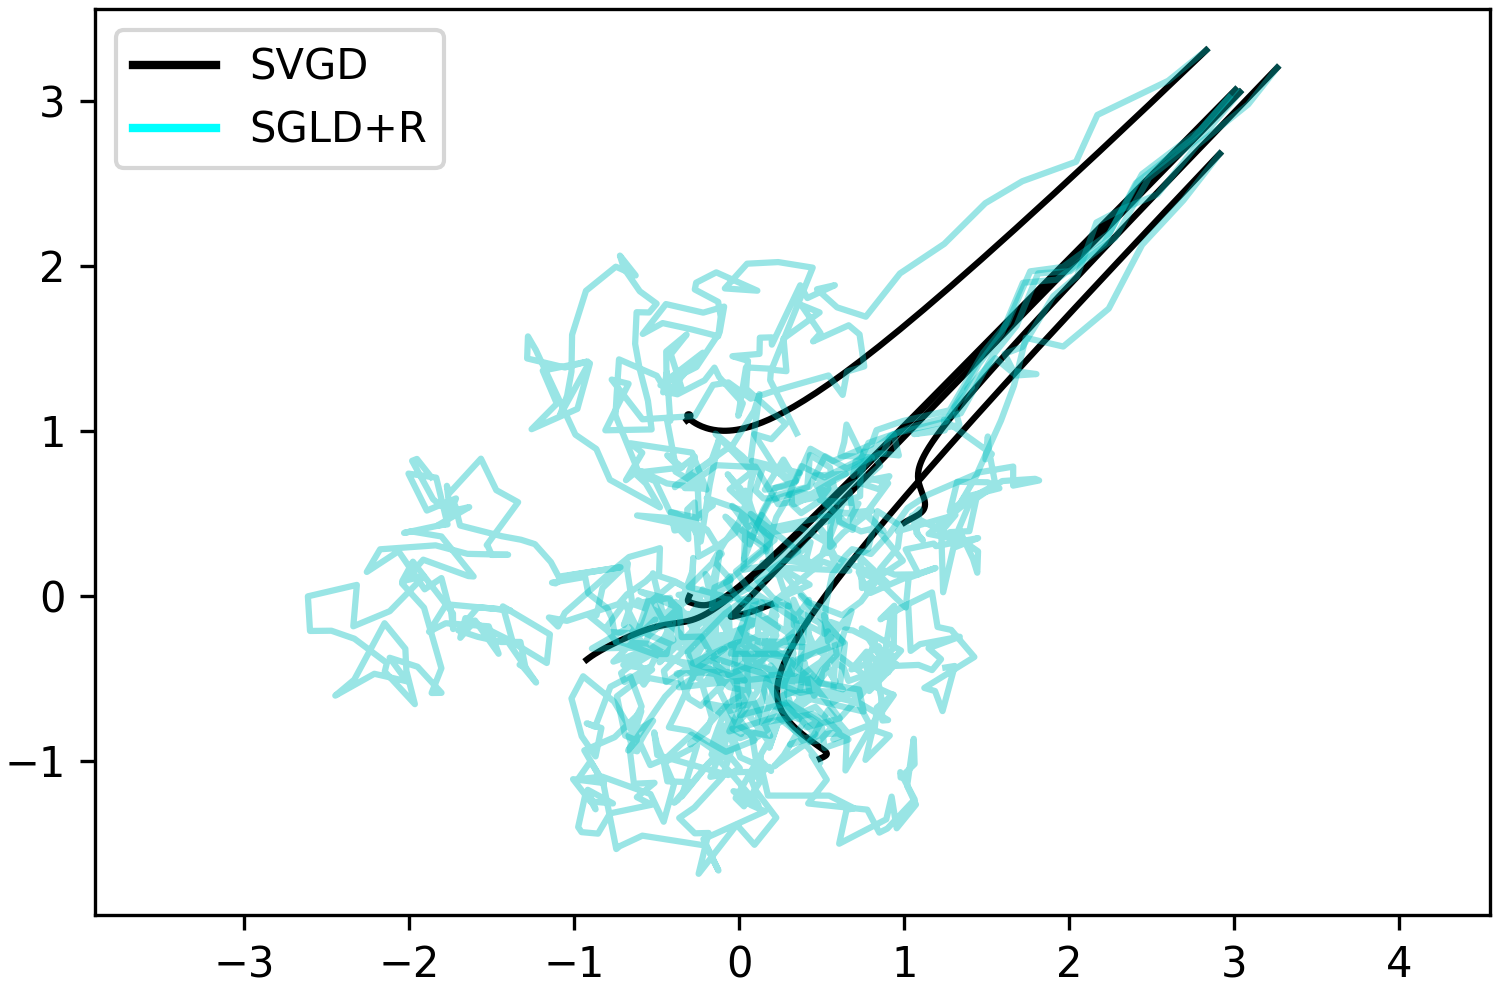
\includegraphics[width=7cm]{img/svgd_vs_sgldr-2.png}
    \qquad
    \begin{tabular}[b]{cccc}\hline
      \textbf{Estimates} & \textbf{SVGD} & \textbf{SGLD+R} & \textbf{Target} \\ \hline
      $\mu$ &  $0.18$ &$\textbf{0.08}$  & 0\\
      $\sigma_{x}$ & $0.70$ & $\textbf{0.90}$ & 1\\
      $\sigma_{y}$  & $0.74$ & $\textbf{0.87}$ & 1\\
    \hline
    \end{tabular}
    \captionlistentry[table]{A table beside a figure}
%    \captionsetup{labelformat=andtable}
    \caption{Trajectories of the compared samplers. The table depicts estimates of quantities of interest for the standard Gaussian target.}
    \label{fig:comp}
  \end{figure}



\subsection{Momentum-based extensions of SG-MCMC samplers with repulsion}\label{sec:momentum}

SGLD+R can be seen as an extension of SGD to incorporate repulsion between particles and the noise term. It is possible to adapt recent developments from the stochastic optimization literature such as Adam, \cite{kingma2014adam}, and propose their equivalent samplers with repulsion.



\paragraph{Momentum} This extension of SGD can be cast as an analogy to the \emph{momentum} in physics, keeping track of previous gradient to prevent oscillations which could slow down learning, \cite{qian1999momentum}. We can frame SGD with momentum as
\begin{align*}
    \bm{z}_{t+1} &= \bm{z}_t - \epsilon_t \bm{m}_t \\
    \bm{m}_{t+1} &= \bm{m}_t - \epsilon_t \nabla \log p(\bm{z}_t),
\end{align*}
where the $\bm{m}_t$ are auxiliary variables.
The previous learning rule can be adapted to our framework by considering an augmented space $\bar{\bm{z}} = (\bm{z}, \bm{m})$. Then, assuming the distribution of $\bm{m}_t$ to be a standard Gaussian, the gradient of the log-density is equal to $-\bm{m}_t$. Next, we set $\mathbf{D} = \mathbf{0}$ and $\mathbf{Q} = \begin{pmatrix}
\mathbf{0} & -\mathbf{I} \\
\mathbf{I} & \mathbf{0}
\end{pmatrix}$ in (\ref{eq:sgmcmc}), arriving at the HMC sampler discussed in Section \ref{sec:infassamp}. 

From this point, we can further augment the latent space, considering $L$ particles $(\bar{z}_1, \ldots, \bar{z}_L)$, to arrive at the SGDm+R sampler. If we rearrange the latent space as $(\bm{z}_1, \ldots, \bm{z}_L, \bm{m}_1, \ldots, \bm{m}_L)$, we may consider the following $\mathbf{Q_K}$ matrix the following one,
$$
\mathbf{Q_K} = \left[
\begin{array}{c|c}
\begin{matrix}
\bm{0} \\
\end{matrix}  & \begin{matrix}
 -\textbf{K} \\
\end{matrix} \\
\hline
\begin{matrix}
\textbf{K}  \\
\end{matrix} & \begin{matrix}
 \bm{0} \\
\end{matrix}
\end{array}
\right],
$$
where $\textbf{K} = \begin{bmatrix}
k(\bm{z}_1, \bm{z}_1) & \ldots & k(\bm{z}_1, \bm{z}_L) \\
\ldots & \ldots & \ldots \\
k(\bm{z}_L, \bm{z}_1) & \ldots & k(\bm{z}_L, \bm{z}_L) \\
\end{bmatrix}$ is the kernel matrix from SVGD. It is straightforward to see that $\mathbf{Q_K}$ is skew-symmetric. Thus we can apply again Proposition 1 to show that SGDm+R is a valid SG-MCMC sampler. The scheme is described in Algorithm \ref{alg:alg2}.

\begin{algorithm}[ht] % 
\caption{Bayesian Inference via SGDm+R}  
\label{alg:alg2}
\begin{algorithmic}
\State {\bf Input:} A target distribution with density function $\pi(\bm{z}) \propto \exp (-H(\bm{z}))$ and priors $p(\bm{z})$ and $p(\bm{m})$.
\State {\bf Output:} A set of particles $\{\bm{z}_i\}_{i=1}^{ML}$ that approximates the target distribution.  
\State Sample initial set of particles from prior: $\bm{z}_1^0, \bm{z}_2^0, \ldots \bm{z}_L^0 \sim p(\bm{z})$.
\State Sample initial set of moments from prior: $\bm{m}_1^0, \bm{m}_2^0, \ldots \bm{m}_L^0 \sim p(\bm{m})$.
\For{each iteration $t$}
\State 
\begin{align*} 
\bm{z}_i^{t+1}  &\gets  \bm{z}_i^t - \epsilon_t \frac{1}{L}\sum_{l=1}^L\big[  k(\bm{z}_l^t, \bm{z}_i^t)  \bm{m}_l^t + \nabla_{\bm{z}_l^t} k(\bm{z}_l^t, \bm{z}_i^t)\big] \\
\bm{m}_i^{t+1}  &\gets  \bm{m}_i^t - \epsilon_t \frac{1}{L}\sum_{l=1}^L\big[  k(\bm{z}_l^t, \bm{z}_i^t)  \nabla_{\bm{z}_l^t} H(\bm{z}_l^t) + \nabla_{\bm{z}_l^t} k(\bm{z}_l^t, \bm{z}_i^t)\big] %+ \bm{\eta}_i^t
\end{align*}
%\State where $\bm{\eta}_i^t$ is the noise for particle $i$ defined as in Eq (\ref{eq:psvgd_mat}).
\State After a burn-in period, start collecting particles: $ \{\bm{z}_i\}_{i=1}^{NL} \gets \{\bm{z}_i\}_{i=1}^{(N-1)L} \cup \{ \bm{z}_1^{t+1}, \ldots,  \bm{z}_L^{t+1} \} $ 
\EndFor
\end{algorithmic}
\end{algorithm}

Next, we show that a similar augmentation can be used to lift more complex optimization schemes to SG-MCMC samplers, one of our contributions.

\paragraph{Adam} The Adam stochastic optimization algorithm has become a \emph{de facto} scheme for optimizing complex non-linear models. In addition to keeping an estimate of the average of past gradients, as in momentum, Adam also keeps track of its variances.
To frame this method in our framework, note that the averages for the gradient can be expressed as
$$
\bm{m}_t = \beta_1 \bm{m}_{t-1} + (1 - \beta_1) \nabla \log p (\bm{z}_t),
$$
where $\beta_1, \beta_2 \in (0, 1)$ are hyperparameters; and, similarly, for the gradient variances,
$$
\bm{v}_t = \beta_2 \bm{v}_{t-1} + (1 - \beta_2) \mbox{diag}(\nabla \log p (\bm{z}_t)_i^2).
$$
Then, the latent state $\bm{z}$ evolves according to
$$
\bm{z}_{t+1} = \bm{z}_t - \epsilon_t \bm{m}_t / \sqrt{\bm{v}_t}.
$$
To frame it in our scheme, with the benefits of interaction between particles, we can consider an augmented space as in the momentum case, $(\bm{z}_1, \ldots, \bm{z}_L, \bm{m}_1, \ldots, \bm{m}_L)$, and adopt $\mathbf{Q_K}$ as before. The difference is that the log-density is now given by $H(\bm{z}, \bm{m}) = \prod_{l=1} ^L \left[ \log p(\bm{z}_l) + \bm{m}_l^{'} \bm{M_l}^{-1} \bm{m}_l \right]$, where $\bm{M_l}$ is the mass matrix for chain $l$, in our case given by
$$
\bm{M_l} = 
\begin{bmatrix}
\sqrt{v_{1,l}} & & \\
 & \ddots & \\
  & & \sqrt{v_{d,l}} 
\end{bmatrix}.
$$
Since $\nabla_{\bm{m}_l} H(\bm{z},\bm{m}) = \bm{m}_l / \sqrt{\bm{v}_l}$, we achieve the same effect of the original Adam, but on a per-chain basis. We call this sampler \emph{Adam plus noise and repulsion}, Adam+NR.





\section{Experiments}\label{sec:experiments}

This Section describes the experiments developed to empirically test the proposed scheme. After the example from Section \ref{sec:relationship}, which compared SVGD and SGLD+R, we focus on confronting SGLD+R with the non-repulsive variant. First, we deal with two synthetic distributions, which offer a moderate account of complexity in the form of multimodality. In our second group of experiments, we explore a more challenging setting, testing a deep Bayesian model over several benchmark real data sets. 

Code for the different samplers is open sourced at \url{https://github.com/vicgalle/sgmcmc-force}. We rely on the library \texttt{jax} \cite{jax2018github} as the main package, since it provides convenient automatic differentiation features with \emph{just-in-time} compilation which is extremely useful in our case for the efficient implementation of SG-MCMC transition kernels.

\subsection{Synthetic distributions} 
The goal of this experiment is to see how well the samples generated through our framework approximate some quantities of interest, which can be analytically computed since the distributions are known. We thus test our proposed scheme with the following distributions. 


\begin{itemize}
\setlength\itemsep{-0.2em}
\item \textbf{Mixture of Exponentials (MoE)}. Two exponential distributions with different scale parameters $\lambda_1 = 1.5, \lambda_2=0.5$ and mixture proportions $\pi_1 = 1/3, \pi_2 = 2/3$. The pdf is
%Probability density function of a mixture of exponentials with $k$ components
$$ 
p(z) = \sum_{i=1}^2 \pi_{i}\lambda_i \exp(-\lambda_i z).
$$
%Where $H(z)$ is the Heaviside step function. It's moments
The exact value of the first and second moments can be computed using the change of variables formula
\begin{equation*}
\mathbb{E} \left[z^n \right] = \sum_{i=1}^2 \pi_{i}\frac{n!}{\lambda_i^n}
\end{equation*}
with $n\in \mathbb{N}$. 
Since $z>0$, to use the proposed scheme, we reparameterize using the $\log$ function. The pdf of the transformation $y = \log(z)$ can be computed using
% \begin{equation*}
% p(y) = \sum_{i=1}^k \pi_{i}\bm{\lambda}_i \exp(-\bm{\lambda}_i \exp(y) + y)
% \end{equation*}
\begin{equation*}
p(y) = p(\log^{-1}(y))|\mbox{D} \log^{-1}(y))|.
\end{equation*}
\item \textbf{Mixture of 2D Gaussians (MoG)}. A grid of $3 \times 3$ equally distributed isotropic 2D Gaussians, see Figure \ref{fig:mog}(d) for the density plot.  We set $\Sigma = \mbox{diag} (0.1, 0.1)$ and place the nine Gaussians centered at the following points:
\begin{align*}
\lbrace (-2,-2), (-2, 0), (-2, 2), (0, -2), \\(0, 0), (0, 2), (2, -2), (2, 0), (2, 2)  \rbrace.
\end{align*}
%\item \textbf{Rough Well}: $U(x) = \frac{1}{2} x^{\top}x + \eta \sum_i \cos (\frac{x_i}{\eta})  $
\end{itemize}
We compare two sampling methods, SGLD with $L$ parallel chains and our proposed scheme, SGLD+R. Note that the main difference between these two sampling algorithms is that for the former $\mathbf{D_K} = \mathbf{I}$, whereas the latter accounts for repulsion between particles. Tables \ref{tab:ess} and \ref{tab:ess2} report the effective sampling size metrics \cite{kass1998markov} for each method using $L=10$ particles. Note that while ESS/s are similar, the repulsive forces in SGLD+R make for a more efficient exploration, resulting in much lower estimation errors. Figures \ref{fig:moe} and \ref{fig:mog} confirm this fact. In addition, even when increasing the number of particles $L$, SGLD+R achieves lower errors than SGLD (see Fig. \ref{fig:moe100}).


\begin{table}[H]
\centering{\small
\scalebox{0.95}{
\begin{tabular}{l|cc|cc}
\hline
& \multicolumn{2} {c} {ESS} & \multicolumn{2} {|c}{ESS/s}  \\
\textbf{Distribution} & {\bfseries SGLD} & {\bfseries SGLD+R} & {\bfseries SGLD}& {\bfseries SGLD+R}  \\
\hline
MoE& $ 44.3 $ & $ \pmb{59.1} $ & $ 51.5 $ & $ \pmb{61.0} $ \\
MoG& $151.3$ &  $ \pmb{169.5}$ &  $\pmb{36.3}$ &  $32.5$  \\
\hline
\end{tabular}
}
}
\caption{Effective sample size results for the two synthetic distributions task}\label{tab:ess}
\end{table}

\begin{table}[H]
\centering{\small
\scalebox{0.95}{
\begin{tabular}{l|cc}
\hline
& \multicolumn{2} {|c}{Error of $\mathbb{E}\left[ X \right]$} \\
\textbf{Distribution} & {\bfseries SGLD}& {\bfseries SGLD+R}  \\
\hline
MoE&  $0.39$  & $\pmb{0.14}$\\
MoG&  $1.42$ & $ \pmb{1.19} $ \\
\hline
\end{tabular}
}
}
\caption{Error results for the two synthetic distributions task}\label{tab:ess2}
\end{table}

For the computation of the error of $\mathbb{E}\left[ X \right]$ in Table \ref{tab:ess}, we sample for 500 iterations after discarding the first 500 iterations as burn-in, and we collect samples every 10 iterations to reduce correlation between samples. For the MoE case, we used 10 particles, whereas for the MoG task, we used 20 particles given the bigger number of modes.


\begin{figure}[ht]
\begin{center}
\minipage{0.45\textwidth}
\hspace{-0.5em}
  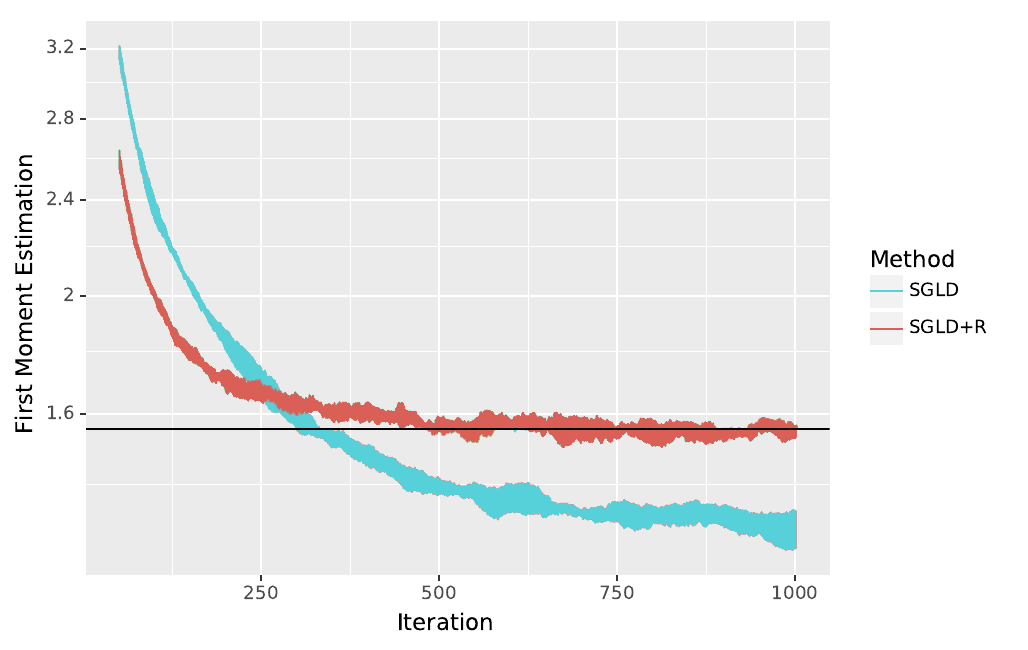
\includegraphics[width=\linewidth]{img/exp1_MOO}
\endminipage\hfill
\minipage{0.45\textwidth}
  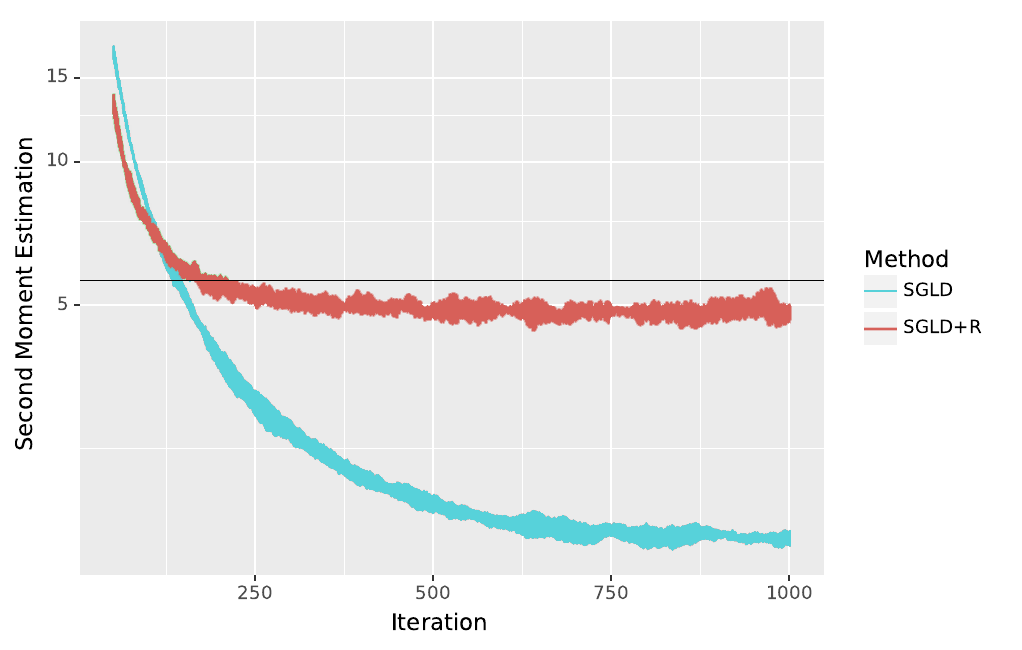
\includegraphics[width=\linewidth]{img/exp2_MOO}
\endminipage
\end{center}
\caption{Evolution of estimation, MoE experiment. Curves plotted for 5 simulations. 10 particles used at each simulation. Black line depicts exact value to be estimated. Left: Estimation of $\mathbb{E}\left[X\right]$. Right: Estimation of $\mathbb{E}\left[X^2\right]$.} \label{fig:moe}
\end{figure}

\begin{figure}[ht]
\begin{center}
\minipage{0.23\textwidth}
\hspace{-0.5em}
  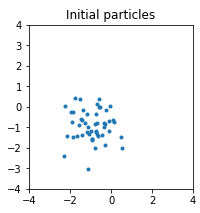
\includegraphics[width=\linewidth]{img/init.png}
\endminipage\hfill
\minipage{0.23\textwidth}
  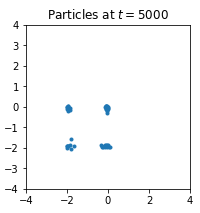
\includegraphics[width=\linewidth]{img/sgld.png}
\endminipage\hfill
\minipage{0.23\textwidth}
  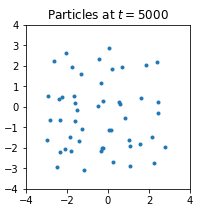
\includegraphics[width=\linewidth]{img/psvgd.png}
\endminipage\hfill
\minipage{0.23\textwidth}
  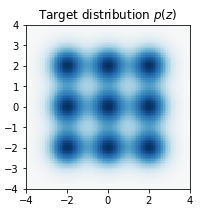
\includegraphics[width=\linewidth]{img/target.png}\label{fig:3x3gauss}
\endminipage
\end{center}
\caption{Evolution of the particles during the MoG experiment. (a) Prior particles. (b) SGLD dyn. (c) SGLD+R dyn. (d) MoG density.}\label{fig:mog}
\end{figure}


\begin{figure}[ht]
\begin{center}
\minipage{0.45\textwidth}
\hspace{-0.5em}
  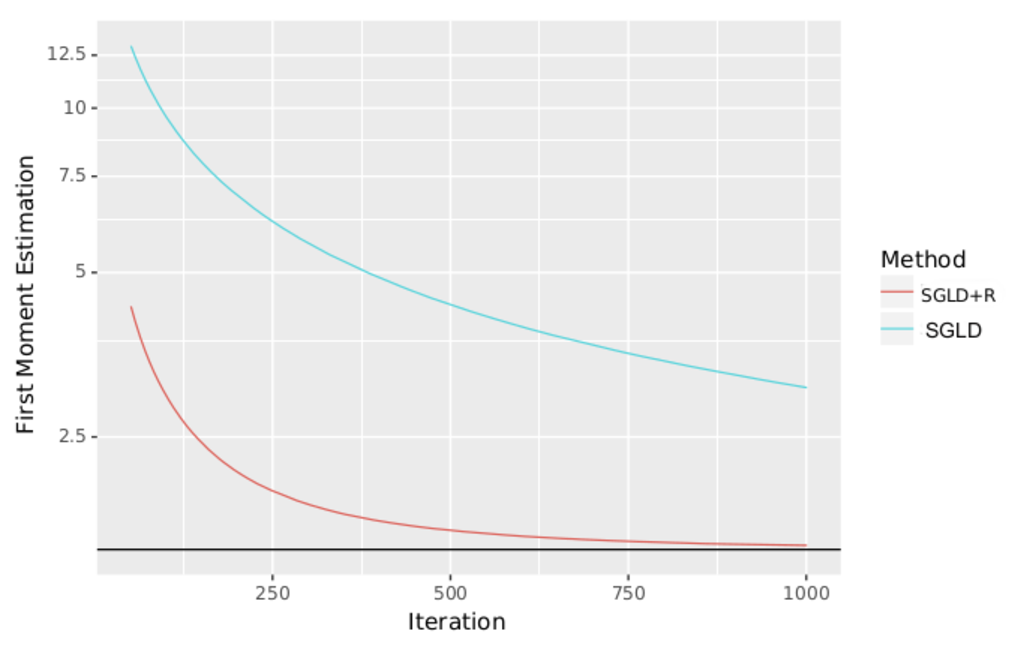
\includegraphics[width=\linewidth]{img/exp1.pdf}
\endminipage\hfill
\minipage{0.45\textwidth}
  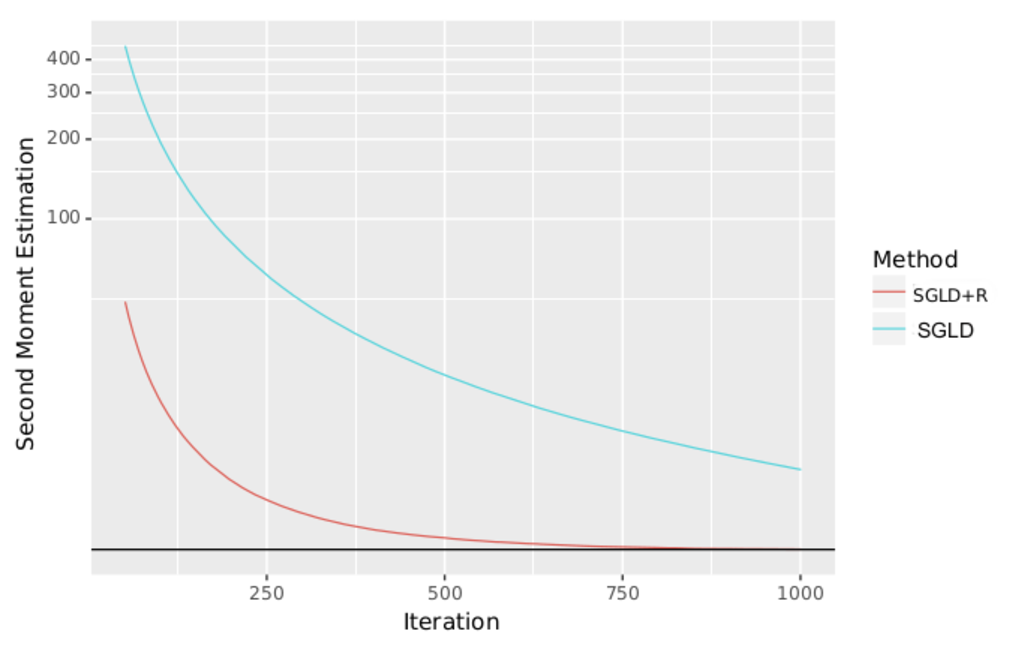
\includegraphics[width=\linewidth]{img/exp2.pdf}
\endminipage
\end{center}
\caption{Evolution of estimation during the MoE experiment. 100 particles are used. Black line depicts the exact value to be estimated. Left: Estimation of $\mathbb{E}\left[X\right]$. Right: Estimation of $\mathbb{E}\left[X^2\right]$.}\label{fig:moe100}
\end{figure}




\subsection{Bayesian Neural Network} 
We test the proposed scheme in a suite of regression tasks using a feed-forward neural network with one hidden layer with 50 units and ReLU activation functions. The goal of this experiment is to check that the proposed samplers scale well to real-data settings and complex models such as Bayesian neural networks. The datasets are taken from the UCI repository, \cite{Lichman:2013}. We use minibatches of size 100. %but while we use the same experimental setting as \cite{liu2016stein}, we use SGD instead of Adagrad, since it is not clear that Proposition 1 can be extended to the non-SGD case. 
As before, we compare SGLD and SGLD+R, reporting the average root mean squared error and log-likelihood over a test set in Table \ref{tab:bnn} and Table \ref{tab:bnn2}. We observe that SGLD+R typically outperforms SGLD. During the experiments, we noted that in order to reduce computation time, during the last half of training we could disable the repulsion between particles without incurring in performance cost.

The learning rate $\epsilon$ was chosen from a grid $\{1e-5, \ldots, 1e-3 \}$ validated on another fold. The number of iterations was set to 2000 in every experiment. As before, to make predictions we collect samples every 10 iterations after a burn-in period. 20 particles were used for each of the tested datasets.

\begin{table}[H]
\centering{\small
\scalebox{0.95}{
\begin{tabular}{l|cc}
\hline
& \multicolumn{2} {c} {Avg. Test LL}  \\
\textbf{Dataset} & {\bfseries SGLD} & {\bfseries SGLD+R}  \\
\hline
Boston&  $ -2.551\pm 0.018$ & $ -2.575 \pm 0.007$ \\
%Concrete&  & & & & & \\
%Energy&  & &  &  &  & \\
Kin8nm&  $0.826 \pm 0.005$ & $0.831 \pm 0.006$  \\
Naval&  $3.379\pm 0.011$ & $ \pmb{3.428 \pm 0.019} $  \\
%Combined&  &  & & & & \\
Protein&   $-2.991 \pm 0.000 $ & $\pmb{-2.987 \pm 0.001} $ \\
Wine&  $ -0.765 \pm 0.008 $ & $ \pmb{-0.750 \pm 0.007}$   \\
Yacht&  $-1.211 \pm 0.020   $ & $-1.172 \pm 0.026 $  \\
%Year&  & &  &  & & \\
\hline
\end{tabular} 
}
}
\caption{Log-Likelihood results for the BNN experiments}\label{tab:bnn}
\end{table}

\begin{table}[H]
\centering{\small
\scalebox{0.95}{
\begin{tabular}{l|cc}
\hline
& \multicolumn{2} {c} {Avg. Test RMSE}  \\
\textbf{Dataset} & {\bfseries SGLD} & {\bfseries SGLD+R}  \\
\hline
Boston& $ 2.392 \pm 0.018$ & $ \pmb{2.295 \pm 0.017}$  \\
%Concrete&  & & & & & \\
%Energy&  & &  &  &  & \\
Kin8nm& $0.104 \pm  0.001  $ & $0.104 \pm 0.001$  \\
Naval& $0.008 \pm 0.000$ & $0.008 \pm 0.000$  \\
%Combined&  &  & & & & \\
Protein& $4.810 \pm 0.003$ & $\pmb{4.794 \pm 0.003} $  \\
Wine& $0.522 \pm 0.004$ & $\pmb{0.514 \pm 0.004}$  \\
Yacht& $0.942 \pm 0.015$ & \pmb{$0.894 \pm 0.029 $}   \\
%Year&  & &  &  & & \\
\hline
\end{tabular} 
}
}
\caption{Root Mean Squared Error results for the BNN experiments}\label{tab:bnn2}
\end{table}

%%%%%%%%%%%%%%%%%%%%%%%%%%%%%%%%
\subsection{Adversarial robustness}

The last set of experiments aims to compare the different momentum-based approaches from Section \ref{sec:momentum}. We study a slightly more complex task than the ones in the previous Section, by studying the robustness of a deep neural network against adversarial examples \cite{goodfellow2014explaining} in the MNIST digit recognition dataset \cite{MNIST}.

We follow a similar setting to \cite{li2017dropout}, since it is hypothesized that the uncertainty from Bayesian neural networks helps against adversarial attacks. First, we generate an attacked dataset using the \emph{fast gradient sign method} (FGSM) from \cite{goodfellow2014explaining}. This attack generates an adversarial perturbation following
$$
x' = x - \eta\,\mbox{sign}(\nabla_x \max_y \log p(y|x))
$$
for a step size $\eta$ that measures attack strength.

The model used for attack generation is a fully-connected network with three hidden layers and 1000 units each with ReLU activations. Then, we test these perturbations on the same network, but trained using SGLD, SGLD+R and Adam+NR, respectively. Figure \ref{fig:attacks} depicts the attack evaluation curves for these inference techniques. As can be seen, Adam+NR in clearly superior in the low attack strength regime compared to the non-momentum counterpart. However, when the attack strength increases, the accuracy of both methods decay to similar levels.



\begin{figure}[h]
    \centering
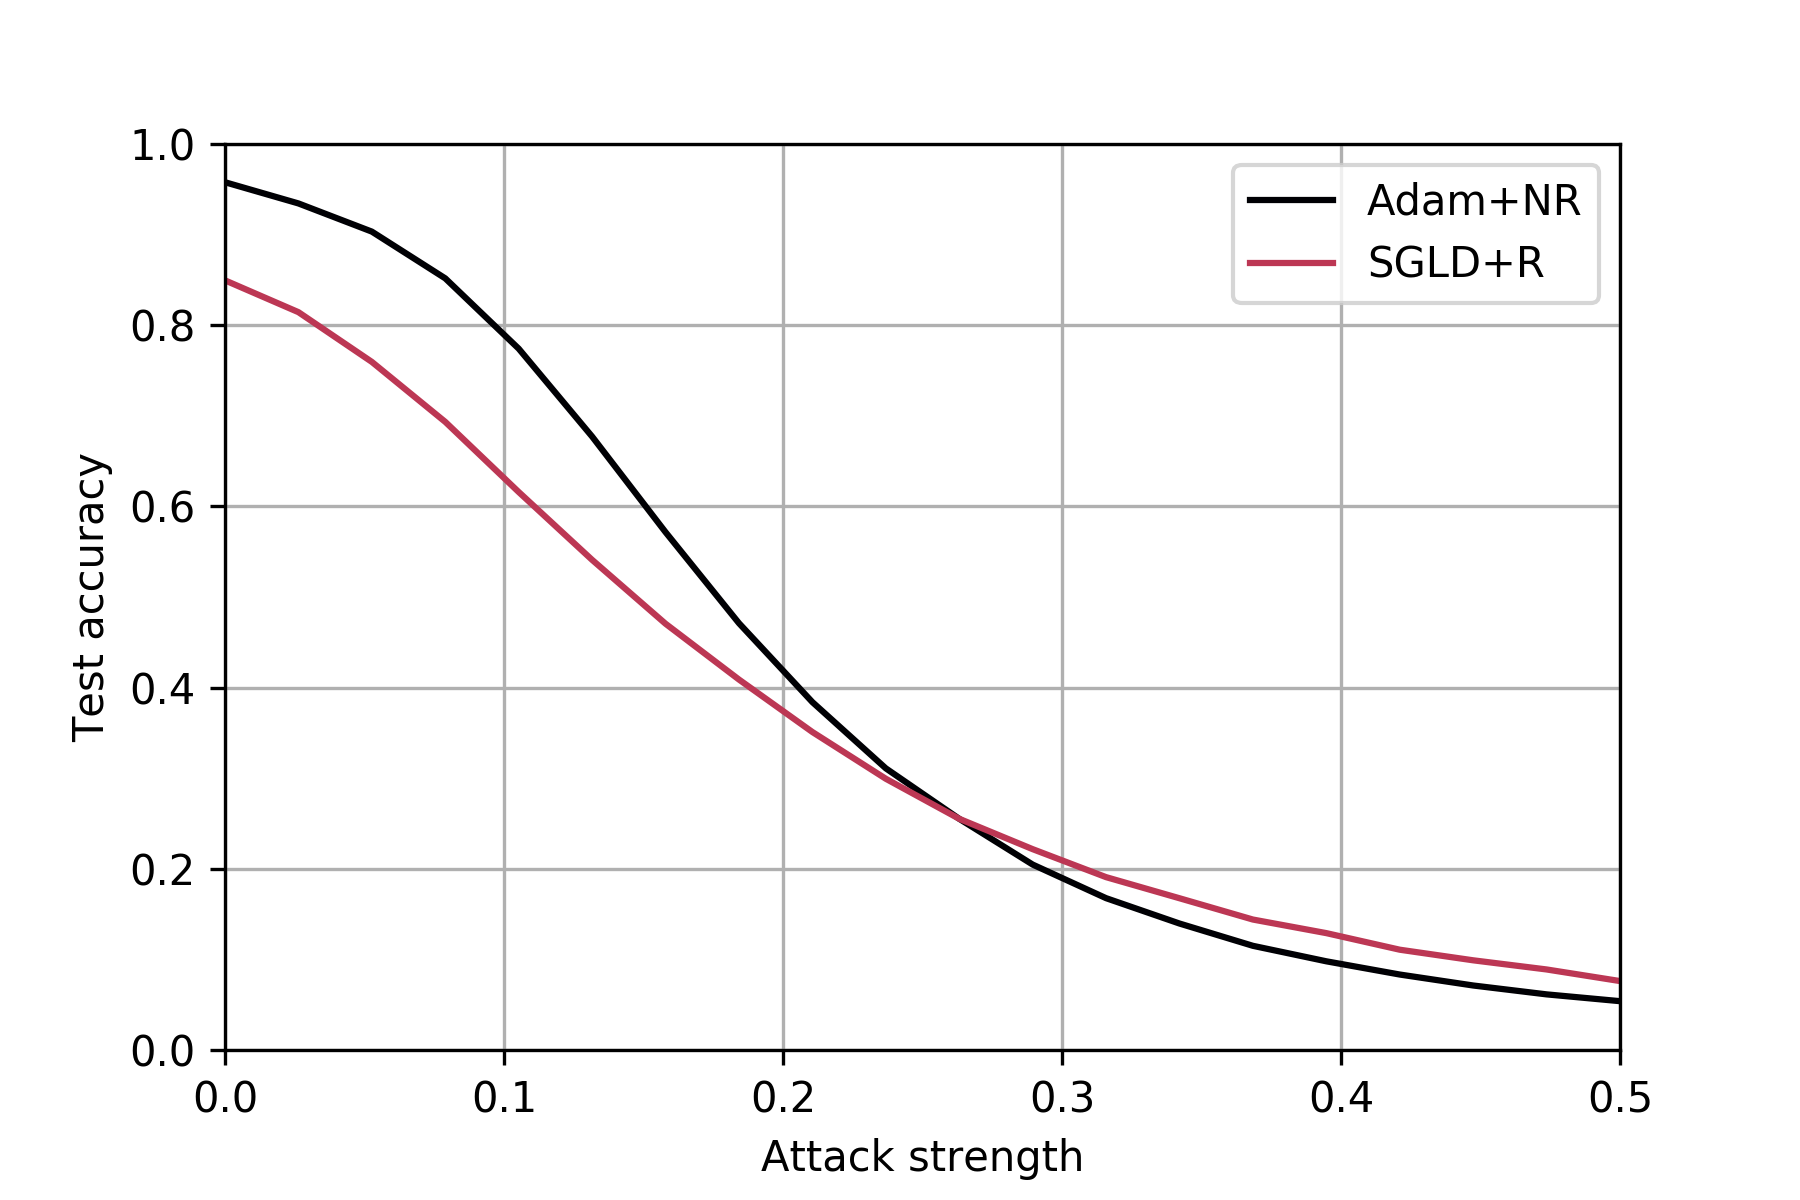
\includegraphics[width=0.5\textwidth]{img/adv-2}
    \caption{Accuracy for various values of attack strengths under the FGSM attack.}\label{fig:attacks}
\end{figure}




%%%%%%%%%%%%%%%%%%%%%%%%%%%%%%%%%%

\section{Conclusions and further work}\label{sec:conclusion}

This paper shows how to generate new SG-MCMC methods, such as SGLD+R and Adam+NR, consisting of multiple chains plus repulsion between the particles. Instead of a naive parallelization, in which a particle from a chain is agnostic to the others, we showed how it is possible to adapt another method from the literature, SVGD, to account for a better exploration of the space, avoiding collapse between particles. We also showed how momentum-accelerated extensions of SGD can be used as SG-MCMC samplers, while also being compatible with the extension to repulsive forces between parallel chains. Our 
experiments show that the proposed ideas improve efficiency when dealing 
with large scale inference and prediction problems in presence of many 
parameters and large data sets.

Several avenues are open for further work. Here we discuss only several promising ones. First, with a very large particle regime ($L >> 100$) there is room to use approximating algorithms such as Barnes-Hutt to keep the computational cost tractable.
Secondly, we used the RBF kernel in all our experiments, but a natural 
issue to address would be to define a parameterized kernel $k_{\theta} (z_i, z_j)$ and learn the parameters $\theta$ on the go to optimize the ESS/s rate, using meta-learning approaches such as the one proposed in \cite{gallego2019vis} for the SGLD case.
When dealing with shallow networks in comparatively small scale problems
\cite{Muller} dealing with acceptance Metropolis steps was crucial, for example,
when focusing on architecture selection; incorporating such steps
to the proposed approaches could be beneficial.



\section{Introduction}
Bayesian inference and prediction in large, complex models, such as in 
deep neural networks or stochastic processes, remains an elusive problem \cite{blei2017variational,insua2012bayesian,alquier2020approximate}.
%
%as in 
%Accurate and efficient uncertainty estimation is becoming increasingly relevant in the Machine Learning community. As current models, such as those grounded in deep learning \cite{SCHMIDHUBER201585}, become more and more complex, traditional uncertainty estimation techniques become obsolete, thus the growing interest in developing newer approximation frameworks.
%
%One of the most popular and flexible paradigms to perform uncertainty estimation is provided by Bayesian statistics \cite{gelmanbda04}. Consider a joint probability model of latent variables and parameters $z$ and observations $x$,
%$$
%p(x,z) = p(z)p(x|z). 
%$$
%Under the Bayesian paradigm, the latent variables govern the distribution of the observed data. A Bayesian probabilistic model draws the latent variables or parameters from some prior distribution $p(z)$ and relates them to the observations via the likelihood probability $p(x|z)$. The machine learning and artificial intelligence communities are pervaded by models that can be expressed naturally through a joint model. Variational autoencoders (VAE) \cite{kingma2013auto} or  hidden Markov models (HMM) \cite{rabiner1989tutorial} are two relevant examples. 
%
%To perform Bayesian inference, we need to condition on the data to compute the posterior distribution, which we can be used to get uncertainty estimates. In complex models, this distribution 
Variational approximations (e.g., automatic differentiation variational inference (ADVI) \cite{kucukelbir2017automatic}) tend to be biased and 
underestimate uncertainty \cite{riquelme2018failure}. 
On the other hand, depending on the target distribution,
%is frequently intractable and requires approximations, such as Monte Carlo methods (e.g.,
Markov Chain Monte Carlo (MCMC) \cite{andrieu2010particle} 
methods, such 
as Hamiltonian Monte Carlo (HMC) \cite{neal2011mcmc}),   
tend to be exceedingly slow  \cite{van2018simple} {in large scale settings with large amounts of data points and/or parameters}. For this reason, in recent years, there has been increasing interest in developing more efficient posterior approximations \cite{nalisnick2016approximate,salimans2015markov,tran2015variational} and inference techniques that aim to be as general and flexible as possible {so that they can be easily used with any probabilistic model} \cite{wood2014new, ge2018t}.

It is well known that the performance of a sampling method depends
heavily on the parameterization used \cite{papaspiliopoulos2007general}. This work proposes
a framework to automatically tune the parameters of a 
MCMC sampler {with the aim of adapting the shape of the posterior, thus~boosting the Bayesian inference efficiency. 
 We deal with a case in which the latent variables or parameters are continuous. Our framework can also be regarded as a principled way to enhance the flexibility of  variational posterior approximation in search of an optimally tuned MCMC sampler;} thus the proposed name of our framework is {the variationally inferred sampler} (VIS).


{

The idea of preconditioning the posterior distribution to speed up the mixing time of a MCMC sampler has been explored recently in \cite{hoffmanneutra,PhysRevLett.121.260601}, where a parameterization was learned before sampling via HMC. Both papers extend seminal work in \cite{parno2014transport} by learning an efficient and expressive deep, non-linear transformation instead of a polynomial regression. However, they do not account for tuning the parameters of the sampler, as introduced in Section \ref{sec:main}, where a fully, end-to-end differentiable sampling scheme is proposed.

The work presented in \cite{rezende2015variational} introduced a general
framework for constructing more flexible variational distributions, called normalizing flows. These transformations are one of the main techniques used to improve the flexibility of current variational inference (VI) approaches and have recently pervaded the approximate Bayesian inference
literature with developments such as continuous-time normalizing flows \cite{chen2018continuoustime} (which extend an initial simple variational posterior with a discretization of Langevin dynamics) or householder flow for mixtures of Gaussian distributions \cite{LIU201943}. However, they require a generative adversarial network (GAN) \cite{goodfellow2014generative} to learn the posterior,
which can be unstable in high-dimensional spaces. We overcome this problem with our novel formulation; moreover, our framework is also compatible with different optimizers, rather than only those derived from Langevin dynamics \cite{10.5555/3122009.3208015}. Other recent proposals create more flexible variational posteriors based on implicit approaches typically requiring a GAN, as presented in \cite{huszar2017variational} and including unbiased implicit variational inference (UIVI)
\cite{pmlr-v89-titsias19a} or semi-implicit variational inference (SIVI) \cite{yin2018semi}. Our variational approximation is also implicit but uses a sampling algorithm to drive the evolution of the density, combined with a Dirac delta approximation to derive an efficient variational approximation, as reported through extensive experiments in Section \ref{sec:exps}.

Closely related to our framework is the work presented in \cite{hoffman2017learning}, where a variational autoencoder (VAE) is learned using HMC. We~use a similar compound distribution as the variational approximation, yet 
our approach allows  any stochastic gradient MCMC to be embedded, %(SG-MCMC) sampler parameterized as $Q_{\eta, T}(z|z_0)$, where $z_0$ is the initial sample, $\eta$ the sampler hyperparameters and $T$ denotes the number of iterations.
 as well as facilitating the tuning of sampler parameters via gradient descent.
Our work also relates to the recent idea of 
sampler amortization \cite{feng2017learning}. 
A common problem with these approaches is that they incur in an additional error---the amortization gap \cite{cremer2018inference}---which we alleviate by evolving a set of particles through a stochastic process in the latent space after learning a good initial distribution,
meaning that %. Hence, the bias generated by 
the initial approximation bias can be significantly reduced.
%after several process iterations % of the process.
A recent related article was presented in~\cite{pmlr-v97-ruiz19a},
which also defined a compound distribution. 
However, our focus is on efficient approximation using the reverse KL %Please define if appropriate 
divergence, %the standard and well understood divergence used in variational inference, 
which allows sampler parameters to be tuned and achieves superior results. Apart from optimizing this kind of divergence, % (better studied than the divergence  use),
the~main point is that we can compute the gradients of sampler parameters %$\eta$ 
(Section \ref{sec:tuning}), whereas in~\cite{pmlr-v97-ruiz19a} the authors only consider a parameterless sampler: % $Q_T(z|z_0)$:
thus, our framework allows for greater flexibility, helping the user
to tune sampler hyperparameters.
In the Coupled Variational Bayes (CVB)~\cite{dai2018coupled} approach,
optimization is in the dual space, whereas
we optimize the standard
evidence lower bound (ELBO). Note that even if the optimization was exact, the solutions would coincide, and it is not clear yet what happens in the truncated optimization case,% (finite $T$), 
other than performing empirical experiments on given datasets. We thus feel that there is room for implicit methods that perform optimization in the primal space 
(besides this, they are easier to implement). Moreover,
the previous dual optimization approach requires the use of an additional neural network (see the paper on the Coupled Variational Bayes (CVB) approach
 or \cite{fang2019implicit}). This adds a large number of parameters and requires another architecture decision. With VIS, we do not need to introduce an auxiliary network, since we perform a ``non-parametric'' approach by back-propagating instead through 
several iterations of SGLD. %Please define if appropriate 
%Thus, the only parameters introduced are the sampler hyperparameters (the step-size in the SGLD case).
Moreover, the lack of an auxiliary network simplifies the design choices.
}


%If we consider a probabilistic program to define a distribution $p(x, z)$, where $x$ are observations and $z$  denote both latent variables and parameters, then we are typically interested in answering queries involving the posterior $p(z | x)$. 

{ Thus, our contributions include a flexible and consistent variational approximation to the posterior,
embedding an initial variational approximation within a stochastic process;} %, together with 
an analysis of its key properties; %(Section \ref{sec:main}); 
    the provision of several strategies for ELBO
    optimization using the previous 
    approximation; and finally, 
    an illustration of its power through relevant complex examples.
    %\item An alternative ELBO function objective formulation, which is a variant of the original one when this new variational approximation is adopted. %(Section \ref{sec:rewriting}).
    %\item A specialization to the case of Bayesian inference in state-space models.% (Section \ref{sec:ss}).
    %\item Variance reduction and reparameterization via delayed sampling to accelerate the sampling process.
    %\item Guide generation (special structure in the warping flow).


 


%BMAML: only SVGD, focus on multiple tasks, custom losses.

\section{Background}
%\section{Background}
Consider a probabilistic model $p(x|z)$ and a prior distribution $p(z)$, where $x$ denotes the observations and $z \in \mathbb{R}^d$ the unobserved latent variables or parameters, depending on the context. Whenever necessary for disambiguation
purposes, we shall distinguish between $z$ for latent variables and $\theta$ for parameters. Our interest is in performing inference regarding the unobserved $z$ by approximating its posterior distribution
$$
p(z| x) = \frac{ p(z)p(x| z) }{ \int p(z)p(x| z) dz} = %\frac{ p(z)p(x| z) }{ p(x) } = 
\frac{p(x, z)}{p(x)}.
$$

The integral assessing the evidence $p(x) = \int p(z)p(x| z) dz$ is typically intractable. %; no general explicit expressions of the posterior are available. 
Thus,~several~techniques have been proposed to perform approximate posterior inference~\cite{alquier2020approximate}.



\iffalse
A probabilistic program defines a probabilistic model $p(x, z)$ that factorizes as
$$
p(x, z) = p(x | z) \prod_{i=1}^n p(z_i | z_{<i}),
$$
where $n$ is the number of latent variables. The previous notation is convenient since it resembles the structure of a generic probabilistic model to sample from $p(x, z)$:
\begin{align*}
    z_1 &\sim p(z_1) \\
    z_2 &\sim p(z_2 | z_{<2}) = p(z_2 | z_1) \\
    &\ldots \\
    z_n &\sim p(z_n | z_{<n}) \\
    x &\sim p(x | z) \\
    \mbox{\texttt{o}}&\mbox{\texttt{bserve }}x,
\end{align*}
where we have $n+1$ sampling statements and then we can condition
 on some observed data. Note that the last factor $p(x|z)$ could be also further factorized. This formulation is sufficiently flexible to describe numerous models typically used in the Machine Learning community, such as the Hidden Markov Model, whose joint probability can be expressed as
$$
p(x, z)
= p(x | z) \prod_{i=1}^\tau p(z_i | z_{i-1}) = \prod_{i=1}^\tau p(x_i |z_i ) p(z_i | z_{i-1}),
$$
for a sequence of $\tau$ observations $x \in \mathbb{R}^\tau$,
and $z_i$ being the hidden state of the observed $x_i$.

Sampling from $p(x,z)$ is tractable as it is just required to run the program forward. However, performing inferences of the form $p(z | x)$ (or some marginal) can be cumbersome, specially in large-scale settings when the number of observations is huge, or the parameters lie in high-dimensional spaces. We next summarise fundamental approaches to deal with this issue.
\fi

%More details about this programs (infinite graph).

\subsection{Inference as Optimization}\label{sec:iasopt}

Variational inference (VI) \cite{kucukelbir2017automatic} tackles the problem of approximating the posterior $p(z | x)$ with a tractable parameterized distribution $q_{\phi}(z|x)$. The goal is to find the parameters $\phi$ so that the variational distribution $q_{\phi}(z|x)$  (also referred to as variational guide
or variational approximation) can be as close as possible to the actual posterior. Closeness is typically measured through 
the Kullback--Leibler 
divergence $KL(q_{\phi } || p)$, reformulated into the ELBO as follows:
\begin{equation}\label{eq:elbo}
\mbox{ELBO}(q) = \mathbb{E}_{q_{\phi}(z|x)} \left[ \log p(x,z) - \log q_{\phi}(z|x)\right],
\end{equation}
\textls[-5]{This is the objective to be optimized,
typically through stochastic gradient descent techniques. To~enhance flexibility, a standard choice
for $q_{\phi}(z|x)$ is a Gaussian 
distribution $\mathcal{N}(\mu_{\phi}(x), \sigma_{\phi}(x))$,
with the mean and covariance matrix defined through a
 deep, non-linear model conditioned on observation $x$.}

%Inference is then performed using a gradient-based optimization routine, leading to variational parameter updates of the form
%\begin{align*}
%\phi_{t+1} = \phi_t + \lambda \nabla_{\phi} \mbox{ELBO}(q),
%\end{align*}
%where $\lambda$ is the learning rate. Stochastic gradient descent (SGD) \cite{hoffman2013stochastic} or some variant of it, such as Adam \cite{kingma2014adam}, are used as the optimization algorithms.

%%%%%%%%%%%%%%%%%%%%%%%%%%%%%%%%%%%%%%
\subsection{Inference as Sampling}

HMC \cite{neal2011mcmc} is an effective sampling method for models whose probability is pointwise computable and differentiable. %HMC uses Hamiltonian dynamics to produce minimally correlated proposals by augmenting the state space of the target distribution $p(z| x)$ with a $d-$dimensional vector $\bm{r}$. The resulting joint distribution is:
%$$
%p(z, \bm{r}| x) = p(z| x)p(\bm{r}),\qquad \bm{r} \sim \mathcal{N}(\bm{0}, \bm{I}).
%$$
%HMC employs two proposals, the first one randomizing $\bm{r}$ (to explore the state space) whereas the second one updates both $z$ and $\bm{r}$ 
%simulating the Hamiltonian dynamics defined through 
%$$
%H(z, \bm{r}) = -\log p(z| x) + \bm{r}^\intercal \bm{r}/2.
%$$
When scalability is an issue, as proposed by the authors in \cite{welling2011bayesian}, a formulation of a continuous-time Markov process that converges to
the target distribution $p(z | x)$ can be used, 
% with $z \in \mathbb{R}^d$. 
which is based~on the Euler--Maruyama discretization of Langevin dynamics
\begin{eqnarray}\label{eq:sgmcmc}
z_{t+1} \leftarrow z_{t} + \eta_t \nabla_{\bm{z}} \log p(x, z_t)  + \mathcal{N}(0, 2\eta_t I),
\end{eqnarray}
where $\eta_t$ is the step size {at time period
$t$, and $I$ is the identity matrix}. The 
required gradient $\nabla \log p(z_t,x)$ can be estimated using mini-batches of data. Several extensions of the original Langevin sampler have been proposed to increase its mixing speed, 
such as in 
\cite{li2016preconditioned,li2016high,abbati2018adageo,gallego2018stochastic}. We refer to these extensions as stochastic gradient MCMC samplers (SG-MCMC) \cite{ma2015complete}.



%%%%%%%%%%%%%%%%%%%%%%%%%%%%%%%%%%%%%%%%%





%%%%%%%%%%%%%%%%%%%%%%%%%%%%%%%%%%%%%%%%%%%%%%%%%%%%
%\section{the Variationally Inferred Sampling (Vis) Framework}\label{sec:main}
\section{A Variationally Inferred Sampling Framework}\label{sec:main}


In standard VI, the variational approximation %$q_\phi(z|x)$
is analytically tractable and typically chosen as a factorized Gaussian, as mentioned above. {However, it is important to note that 
other distributions can be adopted as long as they 
are easily sampled and their log-density and entropy values
evaluated. However, in the rest of this paper, we focus on the Gaussian case, as the usual choice in the Bayesian deep learning community.}
%distribution as described in Section \ref{sec:iasopt}. 
Stemming from {this variational approximation}, we introduce several elements to construct the VIS.

Our first major modification of standard VI proposes the use of a more
flexible distribution, approximating the posterior by embedding a sampler through
\begin{equation}\label{eq:q}
q_{\phi,\eta}(z|x) = \int Q_{\eta, T}(z|z_0)q_{0,\phi}(z_0|x)dz_0,
\end{equation}
where $q_{0,\phi} (z | x)$ is the initial and tractable density
$q_{\phi} (z | x)$
(i.e., the starting state for the sampler). % We refer to $q_{\phi,\eta}(z|x)$ as the {\em refined variational approximation}.
We designate this as refined variational approximation.
The conditional distribution $Q_{\eta, T}(z|z_0)$ refers
to a stochastic process parameterized by $\eta$ and 
used to evolve the original density $q_{0,\phi}(z|x)$
for $T$ periods, so as to achieve greater flexibility. Specific 
forms for $Q_{\eta, T}(z|z_0)$
are described in Section 3.1.
{Observe that when $T=0$, no refinement steps are performed and the refined variational approximation coincides with the original one; on the other hand, as 
%, $q_{\phi,\eta}(z|x) = q_{0, \phi}(z|x)$. 
 $T$ increases, the approximation will be closer to the exact posterior, assuming that $Q_{\eta, T}$ is a valid MCMC sampler
 in the sense of \cite{ma2015complete}}.

We next maximize a refined ELBO objective, replacing in Equation (1) the 
original $q_{\phi }$ 
by $q_{\phi, \eta}$:
\begin{equation}\label{eq:ELBO}
\mbox{ELBO}(q_{\phi,\eta}) = \mathbb{E}_{q_{\phi, \eta}(z|x)} \left[ \log p(x,z) - \log q_{\phi, \eta}(z|x)\right]
\end{equation}
\textls[-5]{This is done to optimize the divergence $KL(q_{\phi,\eta}(z|x) ||  p(z|x))$. {{The first term of Equation (\ref{eq:ELBO})}}
requires only being able to sample from $q_{\phi,\eta}(z|x)$; however, the second
term, the entropy
\linebreak $-\mathbb{E}_{q_{\phi,\eta}(z|x)} \left[ \log q_{\phi,\eta}(z | x) \right]$, also requires the evaluation of the evolving, implicit density.
\linebreak Section~\ref{sec:approx} describes efficient methods to approximate this evaluation. As a consequence, performing~variational inference with the refined variational approximation can be regarded as using the original variational guide while optimizing an alternative, tighter ELBO, as~Section~\ref{sec:rewriting}~shows. }
%Depending on the conditional distribution $Q_{\eta, T}(z|z_0)$, the integral (\ref{eq:q}) may be analytically tractable or not. 

%Note that when latent space is structured, for instance when $z = \left(z_A, z_B \right)$ and $\log p(z_A, z_B) = \log p(z_A|z_B) + \log p(z_B)$ we can apply each of the previous strategies to each sub-expression, as we will see in following examples, described in the next sections.
%In this work, we consider alternatives 2 (Section \ref{sec:grad}) and 3 (Section \ref{sec:ss}), and we left alternative 1 for further work.
The above facilitates a framework for learning the sampler parameters $\phi, \eta$ using gradient-based optimization, with the help of automatic differentiation \cite{baydin2017automatic}.
For this, the~approach operates in two phases.
First, in a refinement phase, the sampler parameters are learned in an optimization loop that maximizes the ELBO with the new posterior. After~several iterations, the second phase,
focused on inference, starts.
We allow the tuned sampler to run for
sufficient iterations, as in SG-MCMC samplers.
This is expressed algorithmically as follows.


Refinement phase: 

Repeat the following until convergence:
    \begin{enumerate}
    \item Sample an initial set of particles, $z_0 \sim q_{0,\phi}(z|x)$.
    \item Refine the particles through the sampler, $z_T \sim Q_{\eta, T}(z|z_0)$.
    \item Compute the ELBO objective from Equation (\ref{eq:ELBO}). %, where the last term may be approximated using any of the methods from Section $\ref{sec:approx}$.
    \item Perform automatic differentiation on the objective wrt parameters $\phi, \eta$ to update~them.
\end{enumerate}


Inference phase: 

Once good sampler parameters $\phi^*, \eta^*$ are learned,
    \begin{enumerate}
    \item Sample an initial set of particles, $z_0 \sim q_{0,\phi^*}(z|x)$.
    \item Use the MCMC sampler $z_T \sim Q_{\eta^*, T}(z|z_0)$ as $T \rightarrow \infty$.
    \end{enumerate}


 Since the sampler can be run for a different number of steps depending on the phase, we use the following notation when necessary: VIS-$X$-$Y$ denotes $T = X$ iterations during the refining phase and $T=Y$ iterations during the inference phase.

%Regarding $Q_{\eta, T}(z|z_0)$, we consider the following families of sampling algorithms.

%\subsection{Gradient-Based Sampling Algorithms} \label{sec:grad}
Let us specify now the key elements.

%%%%%%%%%%%%%%%%%%%%%%%%%%%
\subsection{The Sampler $Q_{ \eta, T}(Z|Z_0)$ } \label{sec:grad}

%\subsection{Gradient-Based Sampling Algorithms} \label{sec:grad}
{ As the latent variables $z$ are continuous}, % ($z \in \mathbb{R}^d$),
we evolve the original density $q_{0,\phi}(z|x)$ through a stochastic diffusion process \cite{pavliotis2014stochastic}. To make it tractable, we discretize the Langevin dynamics using the Euler--Maruyama scheme, arriving at the stochastic gradient Langevin dynamics (SGLD) sampler (2). %Should this be "Equation (2)? Please check,
We then follow the process $Q_{\eta,T} (z | z_0)$,
which represents $T$ iterations of the MCMC sampler. 

As an example, for the SGLD sampler $z_t = z_{t-1} + \eta \nabla \log p(x, z_{t-1}) + \xi_{t},$ where $t$ iterates from 1 to $T$. In this case, the only parameter
is the learning rate $\eta$ and the noise is $\xi_t \sim \mathcal{N}(0, 2\eta I)$. %Note that for some models, the gradient $\nabla \log p(x, z_{i})$ is a linear function of $z_i$, so we can compute the exact distribution of $q(z_{i+1})$ from the distribution of $q(z_i)$. In other cases, we approximate the non-analytical terms using the above Delta approximation. %Figure \ref{fig:refined_guide} provides a graphical representation of the variational approximation. 
The initial variational distribution $q_{0, \phi}(z|x)$ is a Gaussian parameterized by a deep neural network (NN). Then, after $T$ iterations of the sampler $Q$ are parameterized by $\eta$, we arrive at $q_{\phi, \eta}$. 

\iffalse
\begin{figure}[ht]
  \begin{center}
\begin{tikzpicture}[x=1.7cm,y=1.8cm]

  % Nodes
\node[latent]    (Z0)      {$Z^0$} ; %
\node[obs, above=of Z0, yshift=-0.5cm]                   (X)      {$X$} ; %
 \node[latent, right=of Z0]    (Z1)      {$Z^1$} ; % 
   \node[const, right=of Z1]    (Zi)      {$\cdots$} ;
   \node[latent, right=of Zi]    (ZT)      {$Z^T$} ;
 
\node[const, left=of X, xshift=1cm]                   (lam)      {$\phi$} ; %

\node[const, below=of Z0, yshift=1cm]                   (mu)      {$\eta$} ; %

   \factor[above=of Z0]     {Z0-f}     {left:NN} {X,lam} {Z0} ; %
    \factor[right=of Z0]     {Z1-f}     {$Q$} {Z0,mu} {Z1} ; %
     \factor[right=of Z1]     {Zi-f}     {$Q$} {Z1,mu} {Zi} ; %
   \factor[right=of Zi]     {ZT-f}     {$Q$} {Zi,mu} {ZT} ; %
\edge {X} {Z0};
\edge {Z0} {Z1};
\edge {Z1} {Zi};
\edge {Zi} {ZT};

\edge {X} {Z0};
\edge {X} {Z1};
\edge {X} {Zi};
\edge {X} {ZT};


%\plate {} { %
%    (Z0)(ZT)(X) %
%  } {$N$} ; %

\end{tikzpicture}
\end{center}
  \caption{Probabilistic graph for the refined variational approximation.}\label{fig:refined_guide}
\end{figure}
\fi

An alternative arises by ignoring the noise $\xi$ \cite{mandt2017stochastic}, thus refining the initial variational approximation using only the stochastic gradient descent (SGD).
 Moreover, we can use Stein variational gradient descent (SVGD) \cite{liu2016stein} or a stochastic version \cite{gallego2018stochastic} to apply repulsion between particles and promote more extensive explorations of the latent space. %The effect of using different samplers is left for future work.

%%%%%%%%%%%%%%%%%%%%%%%%%%%%%%%%%%%%%%%%%%%%%
\subsection{Approximating the Entropy Term}\label{sec:approx}

We propose four approaches for the ELBO optimization 
which take structural advantage of the refined variational approximation.

    \subsubsection{Particle Approximation (VIS-P)} %Directamente aproximar el posterior variacional mediante dirac deltas y meterle la entropia de la gaussiana original
    
    In this approach, we approximate the posterior $q_{\phi,\eta}(z|x)$ by a mixture of Dirac deltas (i.e., we approximate it with a finite set of particles), by sampling $z^{(1)}, \ldots, z^{(M)} \sim q_{\phi,\eta}(z|x)$ and setting 
    $$
    q_{\phi,\eta}(z|x) = \frac{1}{M} \sum_{m=1}^M \delta(z - z^{(m)}).
    $$
    
    { In this approximation, the entropy term in (4) %Equation? 
    is set to zero. Consequently,  the sample converges to the 
    maximum posterior (MAP).} This may be undesirable when training generative models, as the generated samples usually have little diversity. Thus, in subsequent computations, we add to the refined ELBO the entropy of the initial variational approximation, $\mathbb{E}_{q_{0,\phi}(z|x)} \left[ \log q_{0,\phi}(z | x) \right]$, which
    serves as a regularizer alleviating the previous problem. When using SGD as the sampler, the resulting ELBO is tighter than that without refinement,
    as shown in Section \ref{sec:rewriting}. 
    
    
    %OLDE VERSION: We can view the flow $Q_{\eta,T} (z | z_0)$ as a mixture of Dirac deltas (i.e., we approximate it with a finite set of particles). That is, we sample $z^1, \ldots, z^K \sim Q_{\eta,T} (z | z_0)$ and use $\tilde{Q}_{\eta,T}(z| z_0) = \frac{1}{K} \sum_{i=1}^K \delta(z - z^i)$. Thus, that entropy term is zero so $\mathbb{E}_{q_{\phi,\eta}(z|x)} \left[ \log q_{\phi,\eta}(z | x) \right] = \mathbb{E}_{q_{0,\phi}(z|x)} \left[ \log q_{0,\phi}(z | x) \right]$. If using SGD as the sampler, the resulting ELBO is tighter than the one with no refinement (see Section \ref{sec:rewriting}). However, discarding the entropy in the sampling process results in variational approximations that are too concentrated around the MAP solution, and this might be undesirable for training generative models. 
    
    \subsubsection{MC Approximation (VIS-MC)}
     Instead of performing the full marginalization in Equation (\ref{eq:q}), we approximate it with  { $q_{\phi,\eta}(z_T,\ldots, z_0|x) = \prod_{t=1}^T q_\eta(z_t | z_{t-1}) q_{0,\phi}(z_0|x)$; i.e., we consider the joint distribution for the refinement. However, in inference we only keep the $z_T$ values}. The entropy for each factor in this 
    approximation is straightforward to compute. For 
    example, for the SGLD case, we have
    %$$
    %q_\eta(z_t | z_{t-1}) = \mathcal{N}(z_{t-1} + \eta \nabla \log p(x, z_{t-1}), 2\eta I).
    %$$
    {\bf
    $$ 
    z_t = z_{t-1} + \eta \nabla \log p(x, z_{t-1}) + \mathcal{N}(0, 2\eta I),\qquad  t=1, ..., T.
    $$
    }
This approximation tracks a better estimate of the entropy than 
    VIS-P, as we are not completely discarding it; rather, for each $t$, we marginalize out the corresponding $z_t$ using one sample.
    %%%%%%%%%%%%%%%
          \subsubsection{Gaussian Approximation (VIS-G)} 
          This approach is targeted at settings in which it could be helpful to have a posterior approximation that places density over the whole
        $z$ space. In the specific case of using SGD as the inner kernel, we have
\begin{align*}
z_0 &\sim q_{0,\phi}(z_0|x) = \mathcal{N}(z_0 | \mu_\phi(x), \sigma_\phi(x))\\
z_t &= z_{t-1} + \eta \nabla \log p(x, z_{t-1}), \qquad t=1,\ldots,T.
\end{align*}

By treating the gradient terms as points, the refined variational approximation can be computed as
$ q_{\phi,\eta}(z|x) = \mathcal{N}(z | z_T, \sigma_\phi(x))$. Observe 
that there is an implicit dependence on $\eta$ through $z_T$.

    
    %%%%%%%%%%%%%%%%%%%
      \subsubsection{Fokker--Planck Approximation (VIS-FP)} 
      Using the Fokker--Planck equation, we derive 
    a deterministic sampler via iterations of the form
\begin{equation*}
z_{t} = z_{t-1} + \eta (\nabla \log p(x, z_{t-1}) - \nabla \log q_t (z_{t-1})),\qquad  t=1, ..., T{.}
\end{equation*}

Then, we approximate the density $q_{\phi,\eta}(z|x)$ using a mixture of Dirac deltas. A detailed derivation of this approximation is given in Appendix \ref{app:fp}. 


%%%%%%%%%%%%%%%%%%%%%%%%%%%%%%%%%%%%%%%%%%%%%%%%
\subsection{Back-Propagating through the Sampler}\label{sec:tuning}

In standard VI, the variational approximation $q(z|x;\phi)$ is parameterized by $\phi$. The~parameters are learned employing SGD, or variants such as Adam \cite{kingma2014adam}, using the gradient $\nabla_{\phi} \mbox{ELBO}(q)$. We have shown how to embed a sampler inside the variational guide. 
It~is therefore also possible to compute a gradient of the objective with respect to the sampler parameters $\eta$ (see Section \ref{sec:grad}). For instance, we can compute a gradient
$\nabla_{\eta} \mbox{ELBO}(q)$
with respect to the learning rate $\eta$ from the SGLD or SGD processes to search for an optimal step size at every VI iteration. This is an additional step apart from using the gradient $\nabla_{\phi} \mbox{ELBO}(q)$ which is used to learn a good initial sampling distribution.

% THis Section is not ready yet.
%\subsection{Discrete Latent Variables}

\iffalse
Now we assume that the latent variable $z$ takes a finite set of values.
Could we do the same for Categorical variables?  In more detail, we have
\begin{align*}
z_0 &\sim q(z_0 | x) \sim \mathcal{C}at(\lambda(\bm{x})), \\
z_1 &\sim Q(z_1 | z_0), \\
&\ldots \\
z_{T} &\sim Q(z_T | z_{T-1})
\end{align*}
where $Q$ is a transition kernel. If the discrete variables can
take $K$ values, then we can represent $Q$ as a $K\times K$ stochastic
matrix. Note that we reuse $Q$ after every step, and this matrix 
may be parameterized also by $\bm{x}$. Then, we could perform variable elimination to arrive at a refined guide 
$$
q(z_T | \bm{x}) = \sum_{z_{T-1}, \ldots, z_0 } Q(z_T| z_{T-1}) \ldots q(z_0 | \bm{x}).
$$
%In order to define $Q$, we have thought of two options:
%\begin{enumerate}
%    \item Recall with einsum, we can compute $\nabla  \log p(z, \bm{x})$, and then use some sort of projection to the simplex (as its done in Game Theory with the sigmoid/softmax).
%    \item We define a random $Q$, and then use accept steps at each iteration. Then we need to  compute some gradient to update $Q$ (or just the initial distribution).
%\end{enumerate}
Note the similarity with Eq. \ref{eq:q}. Initially we have $q(z_0| \lambda(x)) \sim \mathcal{C}at(\lambda(x))$ so it should make sense that first of all we optimize $KL(p(z_0, x) || q(z_0 | \lambda(x))$, and then a refinement could be beneficial.

In the high-dimensional setting, $z$ might take $K^d$ values, so having a table as before is intractable. Hence, we make use of another parameterization of the transition operator, given by
$$
z_{t+1,d} = (\mu_d + \sigma_d \cdot z_{t,d}) \mod K,
$$
where $\mu_d$ and $\sigma_d$ are autoregressive functions of $z_{t+1}$. Also bipartite setting. Parameterized as neural nets, we can train the transition and reduce the complexity overhead of the previous transition kernel. Gradients wrt flow parameters are computed using the straight-through gradient estimator \cite{bengio2013estimating}.

Since we are in the discrete setting, we can perform exact inference in the refined marginal:

$$
q(z') = \sum_{z} q(z'|z)q(z) = \sum_{z} \delta_{f(z)}(z') q(z) = q(f^{z})
$$
where the last identity holds if the flow function $f$ has inverse. We can use block ciphers to develop alternative flow functions which have an efficient inverse.

Thus, we reduce the complexity from $\mathcal{O}(K)$ to $\mathcal{O}(1)$. This should be one of the emphasis of the paper (also in the continuous case).

%In Pyro, during training we use exact enumeration on discrete sites (via TraceEnum\_ELBO) to marginalize out discrete variables in the guide. In order to then perform inference on discrete variables we need to use:

%\begin{enumerate}
%    \item infer\_discrete to obtain samples or MAP (much faster but not so general).
%    \item enumerating inside the guide: need to run stochastic optimization for each new input data batch.
%\end{enumerate}

%\subsubsection{Gibbs Sampling Algorithms}
%Think about merging with the discrete case (next section), i.e., whether we focus on continuous vs discrete or SGLD vs SMC vs Gibbs... \\

%Now $Q(z|z')$ is a series of samplers from the conditionals $p(z_i | z_{-i}, x)$. Maybe we can embed the discrete case inside here.
\fi


\iffalse
\subsection{State-Space Model Specialization}\label{sec:ss}
The previous framework is particularly useful in large families of state-space models (and by extension, models that exhibit hierarchical and/or temporal structure), mainly through two complementary strategies: i) exact marginalization of some particular terms (i.e., Rao-Blackwellization \cite{murray2018delayed} to reduce the variance); ii) exact computation in linear cases. %State by saying we are working with state-space models of the form $p(x_{1:T}| x_{1:T}, \theta)$, which can be a HMM, a DLM or deep variants.
Recall that a state-space model \cite{hamilton1994state} can be expressed with the following probabilistic model, where the time-step $t$ iterates from 1 to $\tau$:
\begin{align*}
    z_{t+1} &\sim p(z_{t+1} | z_t, \theta_{tr}), \\
    x_{t+1} &\sim p(x_{t+1} | z_{t+1}, \theta_{em}).
\end{align*}
This formulation subsumes many models used in Machine Learning such as Hidden Markov Models (HMMs) or Dynamic Linear Models (DLMs). It is often required to perform inference on the $\theta := (\theta_{em}, \theta_{tr})$ parameters from the transition and observation equations, respectively. We propose to use a variational distribution $q(\theta)$, which will be refined by any sampling method (as described in Section \ref{sec:grad}):
\begin{equation}
\theta \leftarrow \theta + \nabla_{\theta} \log p(x_{1:\tau}|z_{1:\tau},\theta) + \xi.
\end{equation}
Note that for a large class of models (including HMMs and DLMs) we can marginalize out $z_{1:\tau}$ and have reduced variance iterating with:
\begin{equation}\label{eq:dlm_grad}
\theta \leftarrow \theta + \nabla_{\theta} \log p(x_{1:\tau}|\theta) + \xi,
\end{equation}
where the latent variables $z_{1:\tau}$ have been marginalized out using the sum-product algorithm. For linear-Gaussian models we can also compute the exact form of the refined posterior, since all terms in Eq. \ref{eq:dlm_grad} are linear wrt the latent variables $\theta$. However, inference in these linear models is exact by using conjugate distributions, so the proposed framework is more fit to the case of state-space models containing non-linear (or non-conjugate) components. %For these families of models, we resort to use just a gradient estimator of the entropy or the Delta approximation in Section \ref{sec:grad}.
\fi



%State that the approach of VI + SGLD is general, but we focus on the experimental part on SSM models.

%Also mention the reparameterizations to further speed up the learning.

%Is it interesting to also study VI + Gibbs (could also be integrated with the autoconj)?

\iffalse
\subsection{Automatic Rao-Blackwellization}

%Talk about the paper of Birch \cite{murray2018delayed} and Pyro's tensor variable elimination \cite{obermeyer2019tensor}, i.e., lazy evaluation of probabilistic programs.

%This Section displays several techniques that could be (semi-)automatically implemented whithin the framework of delayed sampling, as initially introduced by \cite{murray2018delayed}.

Assume the latent state can be decomposed into $z = \left( z_V, z_M, z_S \right)$, with $z_M$ being latent variables to be summed out, and $z_S$ (resp. $z_V$) variables that appear before (later) $z_M$ in a probabilistic program. The usual MC estimator adopts the form
$$
\hat{Z} = \sum_{n=1}^N \bar{w}^{(n)} p(z_v | z_M^{(n)}, z_S^{(n)}),\qquad z_M^{(n)} \sim p(z_M^{(n)} | z_S^{(n)}),
$$
where $z_R^{(n)}$ have been previously sampled. Alternatively,
we could perform variable elimination (via a particular instantiation of the sum-product algorithm) on $z_M^{(n)}$, arriving through
a Rao-Blackwellized version to
$$
\hat{Z}_{RB} = \sum_{n=1}^N \bar{w}^{(n)} \int p(z_v | z_M^{(n)}, z_S^{(n)})p(z_M^{(n)}|z_S^{(n)}) dz_M^{(n)}.
$$
Since $Var(\hat{Z}_{RB}) \leq Var(\hat{Z}) $ and both are unbiased, we achieve lower mean squared error with the Rao-Blackwellized variant.
\fi


%\section{Analysis of Vis}
\section{Analysis of Vis}

Below, we highlight key properties of the proposed framework.

\subsection{Consistency}

The VIS framework is geared towards SG-MCMC samplers, where we can compute the gradients of sampler hyperparameters to speed up mixing time (a common major drawback in MCMC \cite{graves2011automatic}).
After back-propagating for a few iterations through the SG-MCMC sampler and learning a good initial distribution, one can resort to the learned sampler in the second phase, so standard consistency results from SG-MCMC apply as $T \rightarrow \infty$ \cite{brooks2011handbook}.

\subsection{Refinement of ELBO}\label{sec:rewriting}

 Note that, for a refined guide using the VIS-P approximation and $M=1$ samples, the refined objective function can be written as 
$$
 \mathbb{E}_{q(z_0|x)} \left[ \log p(x, z_0 + \eta \nabla \log p(x,z_0) ) - \log q(z_0 | x)\right]
$$
noting that $z = z_0 + \eta \nabla \log p(x,z_0)$ when using SGD for $T=1$ iterations.
%Decir que es la de VIS-P, así que el término de entropia es el que nosotros metemos a mano
%$$
%\mathbb{E}_{q(z|z_0)q(z_0|x)} \left[ \log p(x, z) - \log q(z|z_0) - \log q(z_0 | x)\right].
%$$
%However, using the Dirac Delta approximation for $q(z|z_0)$ and , we arrive at the modified objective:
This is equivalent to the refined ELBO in (\ref{eq:ELBO}). Since we are perturbing the latent variables in the steepest direction, we show easily that, for a moderate $\eta$, the previous bound is tighter than
$\mathbb{E}_{q(z_0|x)} \left[ \log p(x, z_0  ) - \log q(z_0 | x)\right]$, the one for the original variational guide~$q(z_0 | x)$. This~reformulation of ELBO is also convenient since it provides a clear way of implementing our refined variational inference framework in any probabilistic 
programming language (PPL) supporting algorithmic differentiation.

Respectively, for the VIS-FP case, we find that its 
deterministic flow follows the same trajectories as SGLD: 
based on standard results of MCMC samplers \cite{murray2008notes}, we have 
$$
KL(q_{\phi,\eta}(z|x) ||  p(z|x)) \leq KL(q_{0, \phi}(z|x) ||  p(z|x)).
$$

A similar reasoning applies to the VIS-MC approximation; however, it does not hold for VIS-G since it assumes that the posterior is Gaussian.

\iffalse
\begin{figure}[htp]
\centering
\begin{minipage}[b]{.45\textwidth}
  \centering
    % trace = {arg.name.split(':')[0]: arg for arg in args}
    % trace.update(kwargs)
    % x = call_with_intercept(model, trace,
    %                         align_latent=lambda name: name,
    %                         align_data=lambda name: name,
    %                         *args, **kwargs)
    % kwargs.update({arg.name.split(':')[0]: arg for arg in args})
    %   log_probs.append(tf.reduce_sum(rv.log_prob(rv.value))
\RecustomVerbatimEnvironment{Verbatim}{BVerbatim}{}
\inputminted[fontsize=\scriptsize]{python}{./elbo.tex}
\caption{ELBO computation within a PPL.}
\label{fig:elbo}
\end{minipage}%
\hspace{1em}
\begin{minipage}[b]{.45\textwidth}
  \centering
    % trace = {arg.name.split(':')[0]: arg for arg in args}
    % trace.update(kwargs)
    % x = call_with_intercept(model, trace,
    %                         align_latent=lambda name: name,
    %                         align_data=lambda name: name,
    %                         *args, **kwargs)
    % kwargs.update({arg.name.split(':')[0]: arg for arg in args})
  \RecustomVerbatimEnvironment{Verbatim}{BVerbatim}{}
\inputminted[fontsize=\scriptsize]{python}{./delbo.tex}
\caption{ELBO computation within a PPL.}
\label{fig:delbo}
\end{minipage}
\end{figure}
\fi


%%%%%%%%%%%%%%%%%%%%%%%%%%%%%%%%%%%%%%%%%%%%
\subsection{Taylor Expansion}\label{sec:taylor}

This analysis applies only to VIS-P and VIS-FP.
As stated in Section \ref{sec:rewriting},  within the VIS framework, optimizing the ELBO resorts to the performance of $\max_z \log p(x, z + \Delta z)$, where~$\Delta z$ is one iteration of the sampler; i.e., $\Delta z = \eta \nabla \log p(x, z)$ in the SGD case (VIS-P), \linebreak or  $\Delta z = \eta \nabla (\log p(x, z) - \log q(z))$ in the VIS-FP case. %The analysis from this subsection does not apply to the other approximations from Section \ref{sec:approx}.
For notational clarity, we consider the case $T=1$, 
although a similar analysis
follows in a straightforward manner if more refinement steps are performed.

Consider a first-order Taylor expansion of the refined objective 
$$
\log p(x, z + \Delta z) \approx \log p(x, z) + (\Delta z)^\intercal \nabla \log p(x, z).
$$

Taking gradients %of the first order approximation 
with respect to the latent variables $z$, we arrive at
$$
\nabla_z \log p(x, z + \Delta z) \approx \nabla_z \log p(x,z) + \eta \nabla_z \log p(x,z)^\intercal \nabla_z^2 \log p(x,z),
$$
where we have not computed the gradient through the $\Delta z$ term (i.e., we treated it as a constant for simplification). Then, the refined gradient can be deemed to be the original gradient plus a second order correction. Instead of being modulated by a constant learning rate, this correction is adapted by the chosen sampler. The experiments in Section \ref{sec:exp} 
show that this is beneficial for the optimization as it 
typically takes fewer iterations than the original variant to achieve lower losses. 

By further taking gradients through the $\Delta z$ term, we may tune the sampler parameters such as the learning rate as 
presented in Section \ref{sec:tuning}. Consequently, the next subsection describes two 
differentiation modes.

%{\color{blue} Do you think it is necessary to make it explicit what happens in the general case when the variational approximation is not a Delta?}

\subsection{Two Automatic Differentiation Modes for Refined ELBO Optimization}\label{sec:AD}

%Here we describe how to implement two variants of the ELBO objective. 
For the first variant, 
remember that the original variant can be 
rewritten (which we term Full AD)~as
\begin{equation}
     \mathbb{E}_q \left[ \log p(x, z + \Delta z) - \log q(z + \Delta z | x) \right].
\end{equation}



We now define a stop gradient operator $\bot$ (which corresponds to \texttt{detach} in Pytorch or \linebreak \texttt{stop\_gradient}~in~tensorflow)  that sets the gradient of its operand to zero---i.e.,~$\nabla_x \bot (x) = 0$---whereas in a forward pass, it acts as the identity function---that is, $\bot (x) = x$. With this, a variant  of the ELBO objective (which we term Fast AD) is
\begin{equation}
    \mathbb{E}_q \left[ \log p(x, z + \bot (\Delta z)) - \log q(z + \bot(\Delta z) | x) \right].
\end{equation}

 Full AD ELBO enables a gradient to be computed
 with respect to the sampler parameters inside $\Delta z$ at the cost of a slight increase in computational burden.
 On the other hand, the~Fast AD variant may be useful in numerous scenarios, as illustrated in the experiments.

\subsubsection{Complexity} 
Since we need to back propagate through $T$ iterations of an SG-MCMC scheme, using~standard results of meta-learning and automatic differentiation \cite{franceschi2017forward}, the time complexity of our more intensive approach (Full-AD) is $\mathcal{O}(mT)$, where $m$ is the dimension of the hyperparameters (the learning rate of SG-MCMC and the latent dimension). Since~for most use cases, the hyperparameters lie in a low-dimensional space, the approach is
therefore~scalable.




%\subsection{Connections to Other Approaches}

%In this subsection we sketch connections to other methods that while at first sight may appear distant.


%\subsubsection{Bmaml.}

%Focus on SVGD, other loss.


%\subsubsection{Meta Learning with Variational Smoothing.} We add an entropy term to the initial distribution parameters.

%Further hiperpriors on the other parameters.




%\section{Experiments}\label{sec:exps}
\section{Experiments}\label{sec:exps}

%We first detail the experiments. 

{The following experiments showcase the power of our 
approach as well as illustrating the the impact of various parameters on its performance, guiding their 
choice in practice. We 
also present a comparison with standard VIS
and other recent variants, showing that the increased computational complexity of computing
gradients through sampling steps is worth the gains in flexibility.
Moreover, the proposed framework is compatible with other structured inference techniques, such as the sum--product algorithm, as well as serving to support other tasks such as  classification}.

Within the spirit of reproducible research, 
the code for VIS has been released at %\url{https://github.com/anon3232/vis}.
\url{https://github.com/vicgalle/vis}. 
The VIS framework is implemented with Pytorch \cite{paszke2017automatic}, although we have also released a notebook for the first experiment using Jax to highlight the simple implementation of VIS.
In any case, we emphasize that the approach facilitates 
rapid iterations over a large class of models. 

%%%%%%%%%%%%%%%%%%%%%%%
\subsection{Funnel Density}

We first tested the framework on a synthetic yet complex target distribution. This~experiment assessed whether VIS is
suitable for modeling complex distributions. The~target bi-dimensional density was defined through
\begin{align*}
    z_1 &\sim \mathcal{N}(0, 1.35) \\
    z_2 &\sim \mathcal{N}(0, \exp(z_1)).
\end{align*}

\textls[-5]{We adopted the usual diagonal Gaussian distribution
as the variational approximation. 
For~VIS, we used the VIS-P approximation and refined it for $T = 1$ steps using SGLD. Figure~\ref{fig:funnel} {top} shows the trajectories of the lower bound for up to 50 iterations of variational optimization with Adam: our refined version achieved a tighter bound. The {bottom} figures present  contour curves of the learned variational approximations. Observe that the VIS variant was placed closer to the mean of the true distribution and was more disperse than the original variational approximation, illustrating the fact that the refinement step helps in attaining more flexible posterior approximations.}


\begin{figure}[ht]
\begin{center}
\minipage{0.45\textwidth}
\hspace{-0.5em}
  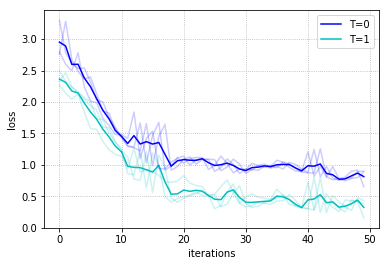
\includegraphics[width=\linewidth]{img/comp_funnel.png}
\endminipage\hfill
\minipage{0.45\textwidth}
  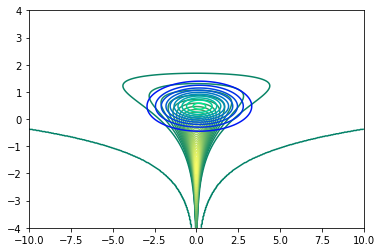
\includegraphics[width=\linewidth]{img/funnel1.png}
\endminipage
\minipage{0.45\textwidth}%
  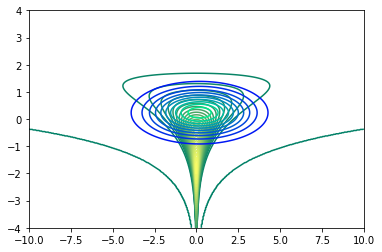
\includegraphics[width=\linewidth]{img/funnel2.png}
\endminipage
\end{center}
\caption{{\textbf{Top}: Evolution of the negative evidence lower bound (ELBO) loss objective over  50 iterations. Darker lines depict means along different seeds (lighter lines). \textbf{Bottom left}: Contour curves (blue--turquoise) of the variational approximation with no refinement ($T=0$) at iteration 30 (loss of $1.011$). \textbf{Bottom right}: Contour curves (blue--turquoise) of  refined variational approximation ($T=1$) at iteration 30 (loss of $0.667$). Green--yellow curves denote target density.}} \label{fig:funnel}
\end{figure}


%%%%%%%%%%%%%%%%%%%%%%%%%%%%%%
\subsection{State-Space  Markov Models}

We tested our variational approximation on two state-space models: one for discrete data and another for continuous observations. These experiments also demonstrated that the framework is compatible with standard inference techniques such as the sum--product scheme from the Baum--Welch algorithm or Kalman filter.
In both models, we performed inference on their 
parameters $\theta$.
All the experiments in this subsection used the Fast AD version (Section \ref{sec:AD}) as it was not necessary to further tune the sampler parameters to obtain competitive results. Full model implementations can be found in Appendix \ref{app:ss}, based on \texttt{funsor} \cite{obermeyer2019functional}, a PPL on top of the \texttt{Pytorch} autodiff framework.



Hidden Markov Model (HMM): The model equations are
\begin{equation}\label{snow}
p(x_{1:\tau} , z_{1:\tau}, \theta) = \prod_{t=1}^\tau p(x_t|z_t,\theta_{em})p(z_t|z_{t-1},\theta_{tr})p(\theta),
\end{equation}
where each conditional is a categorical distribution taking 
five different classes.  The prior is $p(\theta) = p(\theta_{em})p(\theta_{tr})$ based on two Dirichlet distributions that sample the observation and state transition probabilities, respectively. 

Dynamic Linear Model (DLM): The model
equations are as in (\ref{snow}), %Equation?
although the conditional distributions are now Gaussian and the parameters $\theta$ refer to the observation and transition variances. 

 For each model, we generated a synthetic dataset and used the refined variational approximation with $T = 0, 1, 2$. For the original variational approximation to the parameters $\theta$, we used a Dirac delta. Performing VI with this approximation corresponded to MAP estimation using 
 the Baum--Welch algorithm in the HMM case \cite{rabiner1989tutorial} and
 the Kalman filter in the DLM case \cite{zarchan2013fundamentals},
  as we marginalized out the latent variables $z_{1:\tau}$. We used the VIS-P variant since it was sufficient  to show performance gains in this case.%Model details are given in Appendix \ref{app:hmm}. 
 
 Figure \ref{fig:ss} shows the results. The first row reports the experiments related to the HMM, the~second row those for the DLM. We report the evolution of the log-likelihood during inference  in all graphs; the first column reports the number of ELBO iterations, and the second column portrays 
 clock times as the optimization takes place. They confirm that VIS ($T>0$) achieved better results than standard VI ($T=0$) for a comparable amount of time. {Note also  that there was not as much gain when changing from $T=1$ to $T=2$ as there is from $T=0$ to $T=1$, suggesting the need to carefully 
 monitor this parameter. Finally, the~top-right graph for the case $T=0$ is shorter as it requires less clock time.}
 


\begin{figure}[h]

\minipage{0.48\textwidth}
  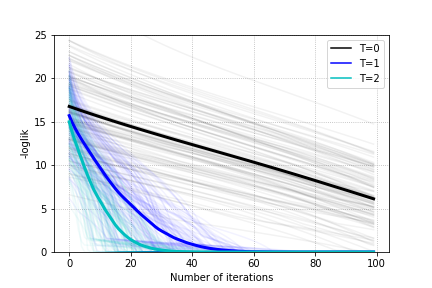
\includegraphics[width=\linewidth]{img/hmm_results.png}
\endminipage
\minipage{0.48\textwidth}
  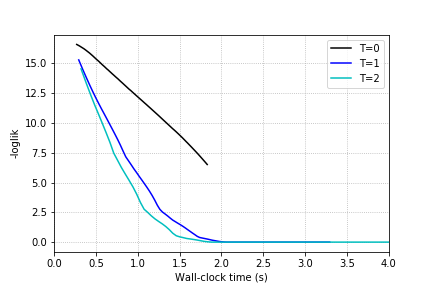
\includegraphics[width=\linewidth]{img/hmm_times.png}
\endminipage\hfill

\minipage{0.48\textwidth}%
  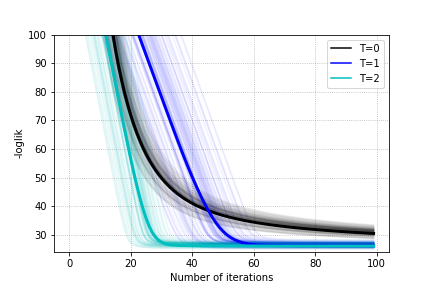
\includegraphics[width=\linewidth]{img/dlm_results.png}
 \endminipage
 \minipage{0.48\textwidth}%
  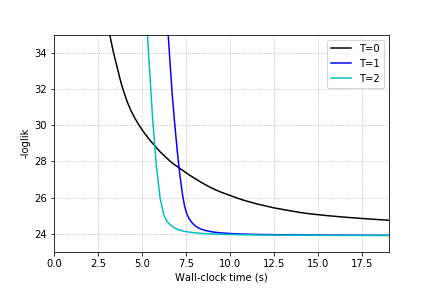
\includegraphics[width=\linewidth]{img/dlm_times.png}
\endminipage
\caption{Results of ELBO optimization for state-space models. \textbf{Top-left} (Hidden Markov Model (HMM)): Log-likelihood against the number of ELBO gradient iterations. \textbf{Top-right} (HMM): Log-likelihood against clock time. \textbf{Bottom-left} (Dynamic Linear Model (DLM)): Log-likelihood against number of ELBO gradient iterations. \textbf{Bottom-right} (DLM): Log-likelihood against against clock time.}\label{fig:ss}%
\end{figure}
   

\subsubsection{Prediction with an HMM} 
With the aim of assessing whether ELBO optimization helps in attaining better auxiliary scores, results in a prediction task are also reported. We generated a synthetic time series of alternating values of 0 and 1 for $\tau=105$ timesteps. We trained the previous HMM model on the first 100 points and report in Table \ref{tbl:preds} the accuracy of the predictive distribution $p(y_t)$ averaged over the final five time-steps. We also report the predictive entropy as it helps in assessing the confidence of the model in its predictions, as a strictly proper scoring rule \cite{gneiting2007strictly}. To guarantee the same computational budget time and a fair comparison, the model without refinement was run for 50 epochs (an epoch was a full iteration over the training dataset), whereas the model with refinement was run for 20 epochs. It can be observed that the refined model achieved higher accuracy than its counterpart. In addition,
it was more correctly confident in its predictions.
\begin{table}[H]

\caption{Prediction metrics for the HMM.}\label{tbl:preds}
\begin{tabular}{c@{\hskip 1.2in}c@{\hskip 1.1in}c@{\hskip 1in}c}
\toprule
   & $\bm{T=0}$                             & $\bm{T=1}$   \\ 
 \midrule
    accuracy          & $0.40$ &  $0.84$ \\
    predictive entropy          & $1.414$ &  $1.056$ \\
    logarithmic score   & $-1.044$ & $-0.682$ \\
 \bottomrule
\end{tabular}
\end{table}

%%%%%%%%%%%%%%%%%%%%%%%%%%%%%%%%%%%%%%%
\subsubsection{Prediction with a DLM}

We tested the VIS framework on Mauna Loa monthly $CO_2$ time-series data \cite{keeling2005atmospheric}. We used the first 10 years as a training set, and we tested over the next 2 years. We used a DLM composed of a local linear trend plus a seasonal block of periodicity 12. %Full model specification are 
%in Appendix \ref{app:ss}.
Data were standardized %As a preprocessing step, we standardize the time series 
to {a mean of zero and standard deviation of one}. To guarantee the same computational budget time, the model without refining was run for 10 epochs, whereas the model with refinement was run for 4 epochs.  Table \ref{tbl:preds_dlm}
reports the mean absolute error (MAE) and predictive entropy. 
In addition, we computed the interval score 
 \cite{gneiting2007strictly}, as a strictly proper scoring rule. As can be seen, for similar clock times, the refined model not only achieved a lower MAE, but also its predictive intervals were narrower than the non-refined counterpart. 

\begin{table}[H]
\centering
\caption{Prediction metrics for the DLM.}\label{tbl:preds_dlm}
\begin{tabular}{c@{\hskip 1.1in}c@{\hskip 1in}c@{\hskip 1in}c}
\toprule
   & $\bm{T=0}$                             & $\bm{T=1}$   \\ 
 \midrule
    MAE          & $0.270$ &  $0.239$ \\

    predictive entropy          & $2.537$ &  $2.401$ \\
    interval score ($\alpha=0.05$) & $15.247$ & $13.461$\\
 \bottomrule
\end{tabular}
\end{table}

%%%%%%%%%%%%%%%%%%%%%%%%%%%%%
\subsection{Variational Autoencoder}

The third batch of experiments showed that VIS 
was competitive with respect to other algorithms from the recent literature, including unbiased implicit variational inference (UIVI~\cite{pmlr-v89-titsias19a}), semi-implicit variational inference (SIVI~\cite{yin2018semi}),  variational contrastive divergence (VCD~\cite{pmlr-v97-ruiz19a}), 
and~the HMC variant from~\cite{hoffman2017learning}, showing that our framework can outperform those approaches in similar experimental settings. 

 To this end, we tested the approach with a variational autoencoder (VAE) model \cite{kingma2013auto}. %Performing efficient and flexible inference in a VAE is useful since it is the building block of more complex models and tasks \cite{chen2018symmetric,bouchacourt2018multi}. 
The VAE defines a conditional distribution $p_{\theta}(x | z)$, generating an observation $x$ from a latent variable $z$ using {parameters $\theta$}. For this task, our interest 
was in modeling the $28 \times 28$ image distributions 
underlying the MNIST %Please define if appropriate 
\cite{lecun-mnisthandwrittendigit-2010} and the fashion-MNIST \cite{xiao2017/online} datasets. To perform inference (i.e., to learn
the parameters $\theta$) the VAE introduces a variational approximation $q_{\phi}(z | x)$. In the standard setting, this distribution is Gaussian; we instead used the refined variational approximation comparing various values of $T$. We used the VIS-MC approximation (although we achieved similar results
with VIS-G) with the Full AD variant given in Section \ref{sec:AD}.

For the experimental setup, we reproduced the setting in \cite{pmlr-v89-titsias19a}. For $p_{\theta}(x | z)$, we used a factorized Bernoulli distribution parameterized by a two layer feed-forward network with 200~units in each layer and relu activations, except for a final sigmoid activation. As a variational approximation $q_{\phi}(z | x)$, we used a Gaussian with mean and (diagonal) covariance matrix parameterized by
two distinct neural networks with the same structure as previously used, except for sigmoid activation for the mean and a softplus activation for the covariance matrix.




%\begin{table}[!ht]
%\centering
%\caption{OLD Test log-likelihood on binarized MNIST and fMNIST.}\label{tbl:iwhvae}
%\begin{tabular}{lcc}
%\cline{1-3}
%\textbf{Method}   & \textbf{MNIST}                             & \textbf{fMNIST}   \\ \cline{1-3}
%\multicolumn{3}{c}{\small Results from \cite{pmlr-v89-titsias19a}}       \\
%    UIVI          & $-94.09$ &  $-110.72$ \\
%    SIVI          & $-97.77$ &  $-121.53$ \\
%    VAE          & $-98.29$ &  $-126.73$ \\
%    \cline{1-3}
    %VIS-10-20 (this paper)     & --- & $\bm{-106.90}$  \\
%    VIS-5-10 (this paper)     & $\bm{-82.47 \pm 0.88}$ & $\bm{-107.32 \pm 1.01}$  \\
    %VIS-0-20 (this paper)    & --- & $-121.11$  \\
%    VIS-0-10 (this paper)     & $-98.13 \pm 0.13$ & $-120.96 \pm 0.58$  \\
    %VAE + RealNVP     & --- & ---  \\
    %VAE + IAF         & --- & --- \\
%    VAE (VIS-0-0)              & $-100.92 \pm 0.09$ & $-125.88 \pm 0.62$ \\
%\end{tabular}
%\end{table}
Results are reported in Table \ref{tbl:vae}. To guarantee 
 fair comparison, we trained the VIS-5-10 variant for 10 epochs, whereas all the other variants were trained for 15 epochs (fMNIST) or 20 epochs (MNIST), so that the VAE's performance was comparable to that reported in \cite{pmlr-v89-titsias19a}. Although VIS was trained for fewer epochs, by increasing the number $T$ of MCMC iterations, we dramatically improved the test log-likelihood. In terms of computational complexity, the~average time per epoch using $T=5$ was 10.46 s, whereas with no refinement ($T=0$), the time was 6.10 s (which was the reason behind our decision to train the refined variant for fewer epochs): a moderate increase in computing time may be worth the dramatic increase in log-likelihood while not introducing new parameters into the model, except for the learning rate $\eta$.
 
 
 \begin{table}[H]
\centering

\caption{Test log-likelihood on binarized MNIST and fMNIST. Bold numbers indicate the best results. UIVI: unbiased implicit variational inference; SIVI: semi-implicit variational inference; VAE: variational autoencoder; VCD: variational contrastive divergence; HMC-DLGM: Hamiltonian Monte Carlo for Deep Latent Gaussian Models; VIS: variationally inferred sampler.}\label{tbl:vae} %
\begin{tabular}{c@{\hskip 0.9in}c@{\hskip 0.8in}c@{\hskip 0.9in}c}
\toprule
\textbf{Method}   & \textbf{MNIST}                             & \textbf{fMNIST}   \\ \midrule
 \multicolumn{3}{c}{Results from \cite{pmlr-v89-titsias19a}}       \\
 \midrule
    UIVI          & $-94.09$ &  $-110.72$ \\
    SIVI          & $-97.77$ &  $-121.53$ \\
    VAE          & $-98.29$ &  $-126.73$ \\
\midrule
 \multicolumn{3}{c}{ Results from \cite{pmlr-v97-ruiz19a}}       \\
 \midrule
    VCD          & $-95.86$ &  $-117.65$ \\
    HMC-DLGM & $-96.23$ & $-117.74$ \\ 
\midrule
    \multicolumn{3}{c}{ This paper}       \\
    \midrule
    %VIS-10-20 (this paper)     & --- & $\bm{-106.90}$  \\
    VIS-5-10     & {$\bm{-82.74 \pm {0.19}}$} & $\bm{-105.08 \pm 0.34}$  \\
    %VIS-0-20 (this paper)    & --- & $-121.11$  \\
    VIS-0-10     & $-96.16 \pm 0.17$ & $-120.53 \pm 0.59$  \\
    %VAE + RealNVP     & --- & ---  \\
    %VAE + IAF         & --- & --- \\
    VAE (VIS-0-0)              & $-100.91 \pm 0.16$ & $-125.57 \pm 0.63$ \\
 \bottomrule
\end{tabular}
\end{table}
Finally, as a visual inspection of the VAE reconstruction 
quality trained with VIS, Figures \ref{fig:reco} and \ref{fig:reco2}, respectively, display 10 random samples of each dataset.
\begin{figure}[h]

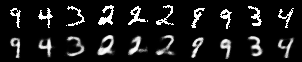
\includegraphics[width=\linewidth]{img/reco_mnist.png}

  \caption{Top: original images from MNIST. Bottom: reconstructed images using VIS-5-10 at 10~epochs.}\label{fig:reco}
\end{figure}
\unskip
\begin{figure}[h]

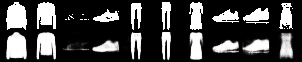
\includegraphics[width=\linewidth]{img/reconstruction_mnist_gauss8_5_10_0_.png}

  \caption{Top: original images from fMNIST. Bottom: reconstructed images using VIS-5-10 at 10~epochs.}\label{fig:reco2}
\end{figure}

%%%%%%%%%%%%%%%%%%%%%%%%%%%%%%%%%%%%%%%%%%%%%%%%%%%%%%%%%%
\subsection{Variational Autoencoder as a Deep Bayes Classifier}\label{sec:exp}
%\section{Concrete Examples}
%Influence Diagrams and Probabilistic Graphical Models
In the final experiments, we investigated whether VIS can deal with more general probabilistic graphical models and also perform well in other inference tasks such as classification.
%Influence diagrams \cite{howard2005influence} are popular representations of decision analysis problems, there being a long history on bridging the gap between influence diagrams and probabilistic graphical models (see \cite{doi:10.1287/opre.36.4.589}, for instance), so developing better tools for Bayesian inference can be transferred to solve influence diagrams.
We explored the flexibility of the proposed scheme to solve inference problems in an experiment with a classification task in a high-dimensional setting %As dataset we use the MNIST \cite{lecun1998gradient} handwritten digit classification task is chosen, in which grey-scale $28 \times 28$ images have to be classified in one of the ten classes $\mathcal{Y} = \lbrace 0, 1, \ldots, 9 \rbrace$.
with the MNIST dataset.
More concretely, we extended the VAE model, conditioning it on a discrete variable\linebreak $y \in \mathcal{Y} = \lbrace 0, 1, \ldots, 9 \rbrace$, leading to a conditional VAE (cVAE). The cVAE defined a decoder distribution $p_\theta(x | z, y)$ on an input space $x \in \mathbb{R}^D$ given a class label $y \in \mathcal{Y}$, latent variables $z \in \mathbb{R}^d$ 
\textls[-15]{and parameters $\theta$. Figure \ref{fig:deep_bayes} depicts the corresponding {probabilistic graphic model}. Additional details regarding the model architecture and hyperparameters are given in Appendix~\ref{sec:detail}.}


\begin{figure}[h]
\centering
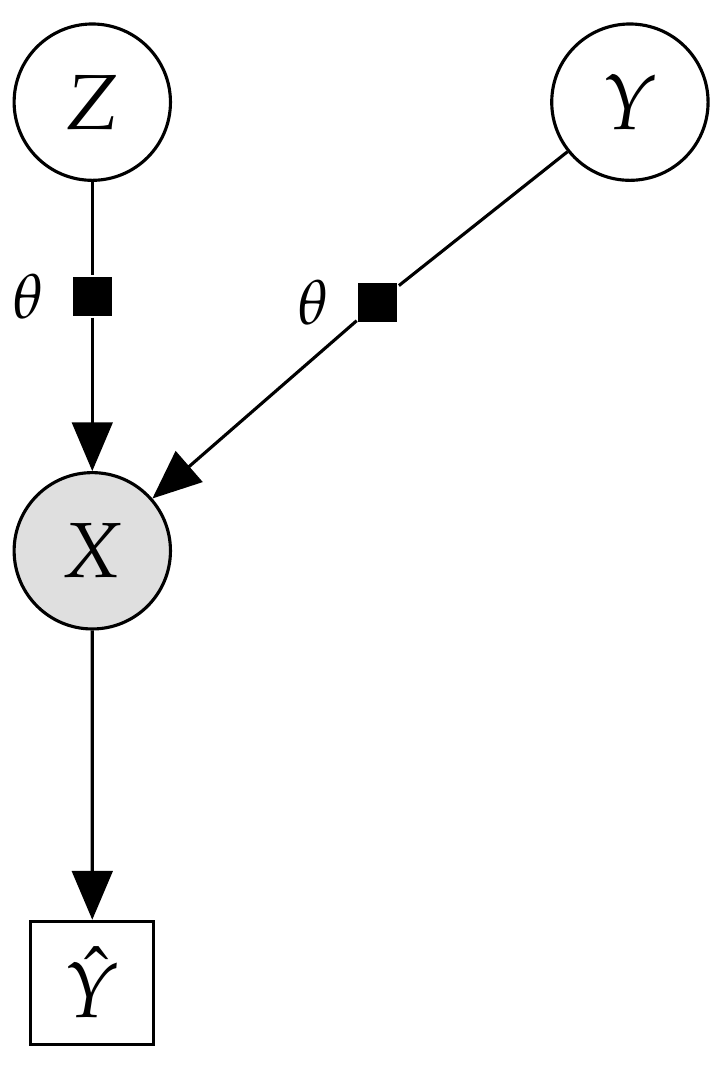
\includegraphics[width=0.4\linewidth]{img/deep_bayes.png}
  \caption{{Probabilistic graphical model} for the deep Bayes classifier.}\label{fig:deep_bayes}
\end{figure}



To perform inference, a variational posterior was learned as an encoder $q_\phi(z|x,y)$ from a prior $p(z) \sim \mathcal{N}(0, I)$.
Leveraging the conditional structure on $y$, we used the generative model as a classifier using the Bayes rule,
\begin{equation}\label{eq:mc_cvae}
p(y|x) \propto p(y)p(x|y) = p(y) \int p_\theta(x|z,y)q_\phi(z|x,y)dz  \approx  \frac{1}{M} \sum_{m=1}^M p_\theta (x | z^{(m)}, y)p(y), 
\end{equation}
where we used $M$ Monte Carlo samples $z^{(m)} \sim q_\phi(z|x,y)$. In the experiments, we set $M = 5$. Given a test sample $x$, the label $\hat{y}$ with the highest probability $p(y|x)$ is predicted.
%assume the existence of a data generating process, $p_{\theta}(x|z,y)$, that generates an instance $x$ belonging to class $y$ and latent variables $z$. The goal of the classifier is, given observed data $x$, predict a label $\hat{y}$ to achieve high utility $U(y, \hat{y})$. We aim at maximizing expected utility. For simplicity, as utility function we assume the standard 1-0 utility, in which $U(y, \hat{y}) = 1$ if $y = \hat{y}$ and $0$ otherwise (though other utility functions are straightforward to implement), thus promoting the classifier to achieve high classification accuracy (i.e., low classification error).
%As it is standard in the supervised learning setting, we split the dataset into a training set, used to learn the variational approximation and model parameters $\theta$, and a testing set, in which we report the mean utility achieved by the classifier for several inference strategies. As dataset, the MNIST \cite{lecun1998gradient} handwritten digit classification task is chosen, in which grey-scale $28 \times 28$ images have to be classified in one of the ten classes $\mathcal{Y} = \lbrace 0, 1, \ldots, 9 \rbrace$. 


For comparison, we performed several experiments changing $T$ in 
the transition distribution $Q_{\eta, T}$ of 
the refined variational approximation. %Note that to solve this ID, apart from learning good variational parameters,it is also required to learn sufficiently good model parameters $\theta$. Hence, the optimization problem to be solved requires alternate updates of the form
%\begin{align*}
%\phi_{t+1} = \phi_t + \lambda \nabla_{\phi} \mbox{ELBO}(q) \\
%\theta_{t+1} = \theta_t + \lambda \nabla_{\theta} \mbox{ELBO}(q).
%\end{align*}
The results are given in Table \ref{tab1}, which reports
the test accuracy at 
end of {the refinement phase}. Note that we are comparing different values of $T$ depending on their use in {refinement or inference} phases (in the latter, the model and variational parameters were kept frozen). The model with $T_{ref} = 5$ was trained for 10~epochs, whereas the other settings were for 15 epochs, to give all settings a similar training time.  Results were averaged over three runs with different random seeds. In all settings, we used the VIS-MC approximation for the entropy term. From the results, it is clear that the effect of using the refined variational approximation (the cases when $T > 0$) is crucially beneficial to achieve higher accuracy. The effect of learning a good initial distribution and inner learning rate by using the gradients $\nabla_{\phi} \mbox{ELBO}(q)$ and $\nabla_{\eta} \mbox{ELBO}(q)$ has a highly positive impact in the accuracy obtained.

On a final note, we have not included the case of only using an SGD or an SGLD sampler (i.e., without learning an initial distribution $q_{0, \phi} (z|x)$) since the results were much worse than those in Table \ref{tab1} for a comparable computational budget. This strongly suggests that, for inference in high-dimensional, continuous latent spaces, learning a good initial distribution through VIS may accelerate mixing time
dramatically.
\iffalse
\begin{table}[H]
\centering

\caption{Results on digit classification task using a deep Bayes classifier.}\label{tab1}
\centering
\begin{tabular}{llccc}
\hline
$T_{tr}$ &  $T_{te}$ & $-\mbox{ELBO}_{tr}$ & $-\mbox{ELBO}_{te}$ & $U_{te}$ (acc.) \\
\hline
0 & 0 & 113.568 & 113.551 & 95.38 \% \\ \hline
0 & 10 & 113.568 & 112.216 &  95.42 \%\\
5 & 10 & \textbf{110.370} & \textbf{109.231} &  \textbf{95.80 \%} \\ \hline
0 & 50 & 113.568 & 110.731 & 95.66 \% \\
10 & 50 & \textbf{110.879} & \textbf{107.702} &  \textbf{99.8 \pm 0.2 \%} \\
\hline
\end{tabular}
\end{table} 
\fi

\begin{table}[H]
\centering

\caption{Results on  digit classification task using a deep Bayes classifier.}\label{tab1}

\begin{tabular}{c@{\hskip 1.4in}c@{\hskip 1.3in}c@{\hskip 1.4in}c}
\toprule
$\bm{T_{ref}}$ &  $\bm{T_{inf}}$ & \textbf{Acc. (Test)} \\
\midrule
0 & 0  & $96.5 \pm 0.5$ \% \\ 
0 & 10 &  $97.7 \pm 0.7$ \%\\
5 & 10 & $ \mathbf{99.8 \pm 0.2}$ \% \\
\bottomrule
\end{tabular}
\end{table}

\iffalse
\subsection{Gaussian Mixture Model}

See \url{http://pyro.ai/examples/gmm.html} for reference.

The model is described as (simplified version)
\begin{align*}
    w &\sim \mathcal{D}irichlet \\
    \sigma &\sim \mathcal{L}ognormal \\
    \mu_k &\sim \mathcal{N}ormal \\
    z_i &\sim \mathcal{C}ategorical(w)  \\
    x_i &\sim \mathcal{N}(\mu\left[z_i\right], \sigma) 
\end{align*}
The variational posterior is specified as $q(w, \sigma, \mu | \bm{x})$, where the discrete variables $z_i$ have been marginalized out (by using TVE in Pyro or sampling in tensorflow-probability). We compare our framework of embedding a sampler inside VI versus just using sampling or just using VI.

Now we list potential augmentations to the model that will be also tested in the experiments:
\begin{enumerate}
    \item $d \sim \mathcal{C}at(w) \rightarrow d \sim \mathcal{C}at(cw)$ (reparameterization as described in Section \ref{sec:reparam}), that should be useful in cases where the resulting $w$ is imbalanced (or there is little data for one cluster).
    \item Instead of the previous continuous reparameterization using $c$, we could add a previous $\mathcal{C}at$ sampling statement leading to the following sequence:
    \begin{align*}
        d_0 &\sim \mathcal{C}at(w_0) \\
        d &\sim \mathcal{C}at(w\left[d_0\right])
    \end{align*}
    where $w$ is now a matrix instead of a vector of probabilities.
    
    
    Benefits: can also perform exact inference since everything is discrete.
\end{enumerate}
\fi


%TODO: repeat VAE experiments using VIS-FP.

\section{Conclusions}
%\section{Conclusion}

In this work, we have proposed a flexible and efficient framework to perform
large-scale Bayesian inference in probabilistic models. The scheme benefits from useful properties and can be 
employed to efficiently perform inference with a wide class of models such as state-space time series, variational autoencoders {and variants such as the conditioned VAE for classification tasks}, defined through continuous, high-dimensional distributions.

The framework can be seen as a general 
approach to tuning MCMC sampler parameters, adapting the initial distributions and learning rate. %We believe the proposed scheme can be successfully applied to Adversarial Risk Analysis \cite{rios2009adversarial}, since MAIDs \cite{koller2003multi} are considered in that setting and it is customary to account for additional uncertainty over an attacker's influence diagram. Our framework paves the way for flexible inference and decision making under uncertainty in these settings, and we will explore this in future work.
Key to the success and applicability of the VIS framework are the ELBO approximations based on the introduced refined variational approximation, which are computationally cheap but convenient. 

Better estimates of the refined density and its gradient may be a fruitful line of research, such as the spectral estimator used in \cite{shi2018spectral}. Another alternative is to use a deterministic flow (such as SGD or SVGD), keeping
track of the change in entropy at each iteration using the change of the variable formula, as in \cite{duvenaud2016early}. However, this requires a costly Jacobian computation, making it unfeasible to combine with our approach of back-propagation through the sampler (Section \ref{sec:tuning}) for moderately complex problems. We leave this for future exploration. {Another interesting and useful line of further research would be to tackle the case in which the latent variables $z$ are discrete. This would entail adapting the automatic differentiation techniques to be able to back-propagate the gradients through the sequences of acceptance steps necessary in Metropolis--Hastings samplers.}

In order to deal with the implicit variational density, it may be worthwhile to consider optimizing the Fenchel dual of the KL divergence, as
 in \cite{fang2019implicit}. However, this requires the use of an auxiliary neural network, which may entail a large computational price compared with our simpler particle approximation.


Lastly, probabilistic programming offers powerful tools for Bayesian modeling.
A~PPL can be viewed as a programming language extended with random sampling and Bayesian conditioning capabilities, complemented with an inference engine that produces answers to inference, prediction and decision-making queries. Examples 
include WinBUGS~\cite{lunn2000winbugs}, Stan \cite{carpenter2017stan} or the recent Edward \cite{tran2018simple} and Pyro \cite{bingham2018pyro} languages. We plan to adapt VIS into several PPLs to facilitate the adoption of the framework.







